%------------------------------------------------------------------------
%
% LaTeX-template for degree projects at LNU, Department of Computer Science
% Last updated by Johan Hagelbäck, Mar 2017
% Linnaeus University
%
% License: Creative Commons BY
%
%------------------------------------------------------------------------

%------------------------------------------------------------------------
%	Settings and configuration
%------------------------------------------------------------------------

\documentclass[a4paper,12pt]{article}

\usepackage[table,xcdraw]{xcolor}
\usepackage[T1]{fontenc}
\usepackage{times}
\usepackage[utf8]{inputenc}
\usepackage{dtklogos}
\usepackage{wallpaper}
\usepackage[absolute]{textpos}
\usepackage[top=2cm, bottom=2.5cm, left=3cm, right=3cm]{geometry}
\usepackage{appendix}
\usepackage{array}
\usepackage{subfig} % Multi-figures

% Change bibliography package, to add last access date
\usepackage[style=ieee]{biblatex}
\addbibresource{referenser.bib}
\usepackage{xpatch}
\xpatchbibdriver{online}
  {\printtext[parens]{\usebibmacro{date}}}
  {\iffieldundef{year}
    {}
    {\printtext[parens]{\usebibmacro{date}}}}
  {}
  {\typeout{There was an error patching biblatex-ieee (specifically, ieee.bbx's @online driver)}}

\usepackage[english]{babel}
\usepackage[colorlinks=true,
            linkcolor=black,
            urlcolor=blue,
            citecolor=black]{hyperref}
\setcounter{secnumdepth}{3}
\setcounter{tocdepth}{3}
\usepackage{sectsty}
\sectionfont{\fontsize{14}{15}\selectfont}
\subsectionfont{\fontsize{12}{15}\selectfont}
\subsubsectionfont{\fontsize{12}{15}\selectfont}

\usepackage{csquotes} % Used to handle citations

% Table padding and styling
\setlength{\arrayrulewidth}{0.5mm}
\setlength{\tabcolsep}{8pt}
\renewcommand{\arraystretch}{1.5}

% Checkmarks
\usepackage{amssymb}
\usepackage{pifont}
\newcommand{\cmark}{\ding{51}}
\newcommand{\xmark}{\ding{55}}

\renewcommand{\thetable}{\arabic{section}.\arabic{table}}
\renewcommand{\thefigure}{\arabic{section}.\arabic{figure}}


%------------------------------------------------------------------------
%
%------------------------------------------------------------------------
\newsavebox{\mybox}
\newlength{\mydepth}
\newlength{\myheight}

\newenvironment{sidebar}%
{\begin{lrbox}{\mybox}\begin{minipage}{\textwidth}}%
{\end{minipage}\end{lrbox}%
 \settodepth{\mydepth}{\usebox{\mybox}}%
 \settoheight{\myheight}{\usebox{\mybox}}%
 \addtolength{\myheight}{\mydepth}%
 \noindent\makebox[0pt]{\hspace{-20pt}\rule[-\mydepth]{1pt}{\myheight}}%
 \usebox{\mybox}}

%------------------------------------------------------------------------
%	Title section
%------------------------------------------------------------------------
\newcommand\BackgroundPic{
    \put(-2,-3){
    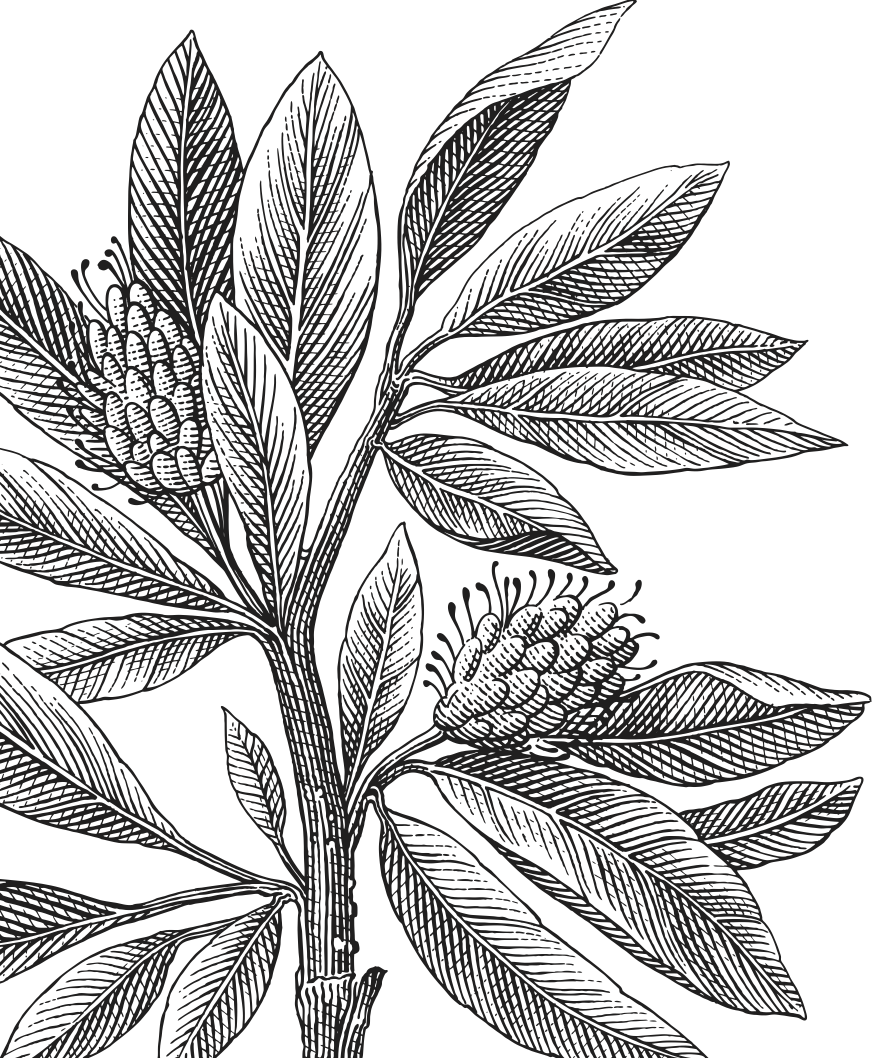
\includegraphics[keepaspectratio,scale=0.3]{img/Other/lnu_etch.png} % Background picture
    }
}
\newcommand\BackgroundPicLogo{
    \put(30,740){
    
\includegraphics[keepaspectratio,scale=0.10]{img/Other/logo.png} % Logo in upper left corner
    }
}

\title{
\vspace{-8cm}
\begin{sidebar}
    \vspace{10cm}
    \normalfont \normalsize
    \Huge Bachelor Degree Project \\
    \vspace{-1.3cm}
\end{sidebar}
\vspace{3cm}
\begin{flushleft}
    \huge The State of Progressive Web Applications\\
    \it \LARGE - an investigation of experience and opinion in the industry
\end{flushleft}
\null
\vfill
\begin{textblock}{6}(10,13)
\begin{flushright}
\begin{minipage}{\textwidth}
\begin{flushleft} \large
\emph{Author:} Adam Elfström\\ % Author
\emph{Supervisor:} Rüdiger Lincke\\ % Supervisor
%\emph{Examiner:} Dr.~Mark \textsc{Brown}\\ % Examiner (course manager)
\emph{Semester:} VT 2021\\ %
\emph{Subject:} Computer Science\\ % Subject area
\end{flushleft}
\end{minipage}
\end{flushright}
\end{textblock}
}

\date{}

\begin{document}
\pagenumbering{gobble}
\newgeometry{left=5cm}
\AddToShipoutPicture*{\BackgroundPic}
\AddToShipoutPicture*{\BackgroundPicLogo}
\maketitle
\restoregeometry
\clearpage
%------------------------------------------------------------------------
%	Abstract
%------------------------------------------------------------------------
\selectlanguage{english}
\begin{abstract}
\noindent The report shall begin with a summary, called abstract. The abstract is a teaser that should summarize the report. The abstract shall not be divided into multiple paragraphs \\
\\
It shall contain:
\begin {itemize}
\item A short description your project’s subject area.
\item A description and motivation for the problems you investigate
\item What methods you have done to address the problems
\item A short summary of your results
\end {itemize}

From reading the abstract the reader should clearly understand what the report is all about. The purpose of the abstract is to make the reader interested in continue reading the report, if it covers something that the reader wants to know more about.
\newline
\newline
\textbf{Keywords:} select three to five keywords for your work here. \textit{Examples: software architectures, adaptive systems, network intrusion detection, ...}
\end{abstract}

\newpage

%------------------------------------------------------------------------
\newpage
\pagenumbering{gobble}
\tableofcontents % Table of contents


\newpage
\pagenumbering{arabic}

%------------------------------------------------------------------------
%
%	Here follows the actual text contents of the report.
%
%------------------------------------------------------------------------


\section{Introduction}
We live in a digital age where mobile phones have become a major part of our daily lives. Modern mobile phones, called smartphones, are predominantly running either the Android or iOS operating systems. Since both platforms have large user bases, companies often need to provide their applications, or apps, on both platforms to not miss out on potential users. The process of developing an app for two distinctly different platforms, while keeping the same functionality and appearance, can be both costly and time-consuming. A solution for this problem is to develop one single app that can run on multiple platforms, a so-called cross-platform app. There are many different options for cross-platform development, but this thesis will focus solely on Progressive Web Applications (PWA). PWAs are built on the same technologies that power normal websites and can be installed on devices like a normal app. PWA stands out from other solutions since it is both relatively old and yet not well-known, despite having huge potential. \{RL: Actually, according to what you write in the next section, PWA is the oldest technology? It was there "first", before Appstore, native applications and hybrid applications like Phone Gap, etc. (besides the applications running natively on the iPhone.)? But then disappeared?\}

\subsection{Background}
In 2007, Steve Jobs revealed a new product from Apple Inc., a mobile phone called the iPhone. During the announcement, he presented their proposed solution to application development on this new mobile platform. By using a web browser and what was at the time state-of-the-art web technologies, developers could create web-based applications that behaved just like native applications \cite{stevejobs_pwa}. However, a year later they introduced an application marketplace, the App Store, which completely replaced this development technique \cite{stevejobs_appstore}. It was not until 2015 that the concept of installable web apps resurfaced in an article published by Google Chrome developer Alex Russel, now named as Progressive Web Applications \cite{russel_pwa}.

A PWA is a cross-platform web application that is in essence a mobile-friendly website that can be installed locally on a device. PWAs are not a new technology, but rather a development technique that adheres to the three major qualities of installability, capability, and reliability \cite{whatarepwas}. The application is installable and is able to run in a separate window instead of only in a browser tab, and can therefore be indistinguishable from a native application. Once installed, it has capabilities much greater than that of a normal website, such as hardware access and proper push notifications. Since its inception, its capabilities have greatly improved, and only a few features are still missing compared to its native counterparts \cite{whatwebcando}. Finally, the application is fast and reliable, regardless of network connection.

Important to note is that there exists a technology similar to PWA, so-called hybrid applications. These are also built on web technologies but wrapped in a native “shell” that allows them to run mobile devices, while PWA’s exclusively use web technologies. Mobile application technologies are further discussed in Chapter 3.

PWA has been called “the future of mobile applications”, that it will take over the mobile landscape \cite{casestudies_mia, futureofweb_claim1}. Even with a potentially promising future, published research on PWA is mainly about a small number of topics, such as its performance and size in comparison to native applications. It proves a challenge to find research related to topics such as the rate of adoption, how widespread the knowledge about the technique is, and general insights into the attitudes towards the technique in the industry. Causes for, and solutions to, issues related to these areas are as you might expect also mostly absent because of this.

\subsection{Related Work}
In 2016, Steczko investigated the differences that exist between native and cross-platform development. He interviewed several companies about their experiences and opinions on the two development alternatives, concluding that the preferred option was native but that both alternatives have their pros and cons \cite{thesis_steczko}. Cross-platform development in a general sense was investigated, but since PWA as a mobile application development technique was almost unknown at the time, it is never mentioned in the report.

In 2020, Olsson and Gustafsson investigated the differences between PWA and native development, extending the work done four years prior by Steczko by conducting similar interviews but instead focusing on PWA rather than general cross-platform development. They also extended the research by using a tool to determine the rate of adoption in Swedish companies, concluding that PWA is drastically under-utilized \cite{thesis_sverige}.

Many other case studies direclty compare a PWA with a native or web app counterpart. For the comparison with web apps, the studies mainly highlight that the initial speed at which the application loads was greatly reduced and that user retention was increased. When comparing to native counterparts, the main advantage was a drastic reduction in app size \cite{casestudies_mia, thesis_pwa_2017, casestudies_google_1, casestudies_google_2, realize_native_with_pwa}.

Thacker and Dharani mention that due to the capabilities of PWA not differing meaningfully from native, the adoption of the technique is expected to rise. They also mention that PWAs are not yet widely known by end-users \cite{realize_native_with_pwa}.

Majchrzak et al. discuss the possibility of PWA becoming the “Definite Approach to Cross-Platform Development”, meaning that PWA would replace all other cross-platform technologies in the future. While a definite conclusion was not drawn, they discussed many different aspects of PWAs in great detail and gave opportunities for research on the topic to further fill the existing knowledge gaps \cite{pwa_definite_approach}.

In a usability test by Sedkowska, native social media applications that also had a PWA alternative were compared and concluded that the participants slightly favored the PWA alternative but that no major usability differences could be found \cite{thesis_pwa_ux}.

\subsection{Problem Formulation}
The research on the topic of PWA is sparse and not very varied. E.g., it proves somewhat challenging to find papers about the state-of-the-art. Furthermore, previous research indicates that PWA is infrequently used and not as well-known as expected. I.e., the technology seems to be rarely known and thus heavily under-utilized.

To understand why this is the case, we aim to investigate the current state of PWA in the industry and whether it deserves broader utilization by gathering opinions and knowledge from mobile application developers. In order to do so, we answer the research questions in Table \ref{tab:rqs}.

\begin{table}[t]
\centering
\rowcolors{2}{black!10!white!100}{black!2!white!100}
\begin{tabular}{|l|p{12.5cm}|}
\hline
\multicolumn{2}{|c|}{\cellcolor[HTML]{343434}{\color[HTML]{FFFFFF} Research questions}} \\ \hline
RQ 1 & Are the most important characteristics of mobile applications realized by PWA? \\
RQ2 & Do developers experience the same problems described in the literature? \\
RQ 3 & What do developers think about PWA and its future? \\
RQ 4 & What needs to change with PWA to achieve more widespread adoption? \\
RQ 5 & Do customers influence the decision of native vs PWA? \\
RQ 6 & What is the state of PWA coverage in web \& app development in higher education? \\ \hline
\end{tabular}
\caption{All research questions the thesis aims to answer}
\label{tab:rqs}
\end{table}

\subsection{Motivation}
\{RL: not sure if we need this: This thesis can highlight the strengths and weaknesses of PWA and examine what its most prominent issues are today. The opinions and experiences of app developers are also important to present to help the industry drive further development to improve on the technology.\}

Poor knowledge of PWA in the industry can mean a missed opportunity to build the best app for a company’s purpose. The results of the thesis might lead companies to decide to offer PWA as a solution to customers, and be incentivized to further inform customers about the advantages the tech can offer them.

In conjunction with the results from surveying higher education, further knowledge of the underlying causes for the perceived low adoption of PWA in the industry can be gained. The results of this thesis might also incentivize lecturers in higher education to incorporate PWA into their courses, improving the variety of development techniques and technologies taught in higher education, and avoiding failing to meet the needs of industry.

\subsection{Results}
This thesis uses surveys as the method for obtaining data about the current state of PWAs which means that the primary result will be the data collected from said surveys. From an evaluation of this data, conclusions can be drawn about what the state of PWA as a development technique is from the perspective of the industry. The surveys contribute to answering all of the research questions.

We list a ranking of the most common issues with PWA according to the literature. While this list does not on its own answer any research questions, it creates knowledge that is useful particularly when creating the surveys.

Research questions 1 and 4 are further answered by the creation of a checklist containing the most important changes needed for PWAs to achieve more widespread adoption. This checklist is based on a literature study and a survey question that ask developers to rank the importance of different mobile app characteristics and features. See Section 4.2 for more details about the survey questions and Appendix A and B for the full surveys. Since the checklist is created from the survey responses it is therefore validated by the collected real-world data.

\subsection{Scope \& Limitations}
In this thesis, the current state of PWA is investigated by interviewing companies and higher educational institutes about the technique. The numerical rate of adoption in the different countries that are investigated as well as exactly what PWAs are capable of today is not to be investigated.
The investigation is limited by only surveying companies offering mobile application development services. The companies are further limited to be based in one of four different countries (Sweden, USA, Poland, and India). For the educational investigation, only higher educational institutes in Sweden are to be surveyed.

\subsection{Target Group}
The target group of this research is mostly application developers and their employing companies since they get an opportunity to take part in perspectives from other companies in the industry. Another group that might have an interest in the thesis is educators in higher education as they might currently have an interest, or develop one based on the results, in adding something about PWA to their curriculums.

\subsection{Outline}
The rest of this report will have the following structure:
\begin{itemize}
    \item Chapter 2 includes discussions about the scientific approach, research method, and ethical considerations for the project.
    \item Chapter 3 further discusses the existing knowledge gap the thesis investigates and the theoretical background.
    \item Chapter 4 discusses all steps taken when collecting the data.
    \item Chapter 5 presents the collected data.
    \item Chapter 6 contains the analysis of the collected data.
    \item Chapter 7 discusses the findings of the project and whether the problem has been solved. The results are also discussed related to other work in the field.
    \item Chapter 8 contains the conclusions drawn and gives suggestions for future work.
\end{itemize}

\newpage

\section{Method}
\label{Method}
This chapter contains a more detailed description of the scientific methods used for this thesis project. Section 2.1 \{use reference/link in latex\} introduces the project by outlining what methods will be used for which parts of the project and gives an overview of how the project will be carried out. Section 2.2 gives more details about the methods that were introduced in Section 2.1, as well as briefly mentioning what methods were chosen to not be used. Section 2.3 discusses the reliability and validity of the project, by describing what threats exist that might lead to a degradation of the quality of the results and subsequent conclusions drawn from these results. Finally, Section 2.4 discusses ethical considerations for the project, such as how to preserve the anonymity of survey participants.

\subsection{Research Project}
This research project aims to answer questions about the current state of PWA, both in terms of developer’s opinions and in terms of offerings in the education sector. A multimethod approach was chosen for this project, and since the creation of any artifacts apart from the survey are not needed, this approach appears sufficient.

To answer the research questions, the project is split into two major stages that each produce something for the report:

\begin{enumerate}
    \item A literature study will answer some of the questions in the survey for industry, and also produce some of the questions for the survey for universities.
    \item Conducting the surveys will finally allow us to answer our research questions.
\end{enumerate}

Getting an overview of PWA as a technique, and more specifically what problem areas exist, is the first step necessary to create the questions of the surveys. The chosen method for this step is a literature study on scientific research and grey literature which aims to give the knowledge necessary to create the survey. Not all questions are based on the study however; some are purely based on the research questions and the information in Chapter 3 \{also reference in LaTeX, use \textbackslash{label}\{\} and \textbackslash{ref}\{\} \}.

The first step of conducting the survey is the process of selecting which companies to contact for participation. A company fitting for participation must offer a downloadable mobile application and have experience developing a downloadable mobile application. Their primary business might be application development, although this is not a strict requirement. The primary method of finding fitting companies and the correct people in said companies to contact is to use the search function built into the business-to-business (B2B) website Clutch \cite{clutch}. Section 2.2.2 contains more information about the method, while Chapter 4 details the exact steps that were taken in the searching process.

Following the creation of the questions, answers to these must be obtained. The chosen method(s) for this step is to perform a survey by contacting selected companies and introduce the project to them. A questionnaire is to be attached to this introductory message to allow for swift participation. They may choose to answer the survey online directly through the link provided, or through other means if necessary. If a company decides to participate in an alternative way, this might be done by scheduling a phone call in which the survey is instead conducted more in the fashion of an interview. If this is the case, the call will be recorded and its answers later added to the answers given by regular survey participation. The choice of including alternative means of participation is based on a wish to increase the likelihood of companies participating in the study since the companies might have wished to not answer an online form.


\subsection{Research Methods}
The following Sections each describe in more detail the methods chosen.

\subsubsection{Literature Study}
A literature study will initiate the project by providing the information necessary to formulate the questions for the surveys. This study is to be conducted primarily on so-called grey literature, meaning articles written and published by non-academic sources. While some academic literature will be included in the study, it will be a minority because of its relative scarcity.

This method was chosen since it was deemed to be the most effective way of acquiring the information needed. Alternative methods included interviewing experts in the field and conducting case studies about the pros and cons of using the technique. Both of these alternative methods were deemed to not be feasible for this project due to time constraints.

\subsubsection{Surveys}
The industry survey is to be split into two separate parts. The first part contains more general information that non-developers are still able to answer. The second part is only to be answered by developers, as it will contain questions that are directly related to the development process and the experience of the developers. The creation process of the survey questions is described in Chapter 4.

Before the surveys can be conducted, a selection of companies to be participants in the surveys needs to be made. This selection process will include selecting companies from different sectors to improve the diversity of participants, but of note is that this might prove to be ineffective. The reason is that companies from different industries have a differing likelihood of having developed applications in-house, so the end result will most likely still be somewhat one-sided. Companies that have no experience in developing applications in-house are still of interest to this project, as they can still answer the first part of the survey. If a company is willing to participate, they will be asked to forward the survey to the relevant person(s) in the company to answer in their free time. A scheduled phone interview is also possible if necessary.

The survey to be conducted in the education sector will be limited to only include professors from Swedish universities. The ten largest universities in the country will be selected, and then professors from these universities that teach in courses related to web development and design will be contacted.

Surveys were chosen as the primary method for obtaining data since they allow for easier collection of larger amounts of data. Purely doing interviews over the phone, or some other voice-communication medium, require more time and might therefore result in fewer participants. The survey was also deemed more fitting for having a mix of quantitative and qualitative questions, which for this project is desirable.

\subsection{Reliability and Validity}
This section contains discussions of the reliability and validity of the project, with a separate section for the literature study and the interviews.

\subsubsection{Literature Study}
Since the literature study was conducted as a precursor to the construction of the survey material, from which the results could then be derived, it is somewhat important that the material that was studied was of adequate quality. Since the scientific literature on this subject is limited, grey literature needs to be used which can be argued greatly increases the risk of the results having potential problems with validity. Something that decreases this risk is that many sources of grey literature discuss similar aspects of PWA. Since a consensus on what the most important aspects of the technique appear to exist, the use of grey literature becomes easier to justify. The study does not exclusively examine grey literature, as a few scientific sources are also included.

\subsubsection{Surveys}
The results derived from the surveys will most likely suffer from both external validity and have issues with reliability. The process of selecting the companies to contact and the lecturers to contact is completely manual, meaning that the person doing the selections has an impact on which people are contacted. Additional external validity issues arise from the fact that the directory of development companies used for finding companies to contact is owned by a business. This business might for instance change their terms of service two months from now resulting in a massive difference in which companies are included in the directory.

To mitigate the problem of reliability, all steps taken in the process of selecting participants are documented in Chapter 4. The issue of external validity will however be present and would only be completely solved if the directory was fully static and the selection process was fully automated.

As for the survey aimed at the education sector, the selection process is once again not automated. All of the schools listed as being Universities or equivalent in Sweden are considered for participation. Since this list is unlikely to drastically change, the process is much more likely to be replicated. The selection process is limited to Swedish universities only, and only lecturers in courses related to web and/or app development and design are contacted.

\subsection{Ethical Considerations}
All persons participating in the survey will before it begins be briefed on who is behind the survey, why it is being conducted, and how their participation will be anonymous. No participants are forced to take part in this study, their participation is completely voluntary.
The name of all participants, be it individual persons or company names, will not be presented in this report to preserve their anonymity. If any voice interviews are conducted, the recordings of said interviews will be deleted before the end of the project.

Which parties choose to participate in the survey might result in a bias emerging. This is mitigated by only contacting a company asking for only one of their developers to participate, and to contact companies from different countries.

\newpage

\section{Theoretical Background}
This chapter describes in more detail the concepts of responsive web design, mobile applications, and different cross-platform development technologies and techniques. Understanding these concepts and how they related to each other is helpful for understanding the design of the survey and the results it produced.

\subsection{Responsive Web Design}
From a visual perspective, there exist two distinct types of websites; fixed-width websites and responsive websites. Before smartphones became popular, websites were typically designed around a minimum target resolution by using fixed sizes for all its elements, often expressed in a number of pixels \cite{resp_web_2011}. This type of website is not capable of adapting its content to fit screens of different sizes; it stays static regardless of the device that is viewing the site. This causes problems with devices having particularly small screens or large screens since elements containing text might become illegible.

A responsively designed website uses relative sizes for elements, such as percentage widths instead of fixed pixel widths. Responsive websites are therefore fluid and flexible, allowing scaling to both ends of the screen-size spectrum. Additionally, so-called “media queries” are used to further optimize the site and remove issues visible above or below certain screen sizes \cite{resp_web_2011}.

Figure \ref{fig:responsiveness} illustrates how a website uses media queries to optimize its appearance for different devices.

\begin{figure}[h]%
	\centering
	\subfloat[Laptop view]{\fbox{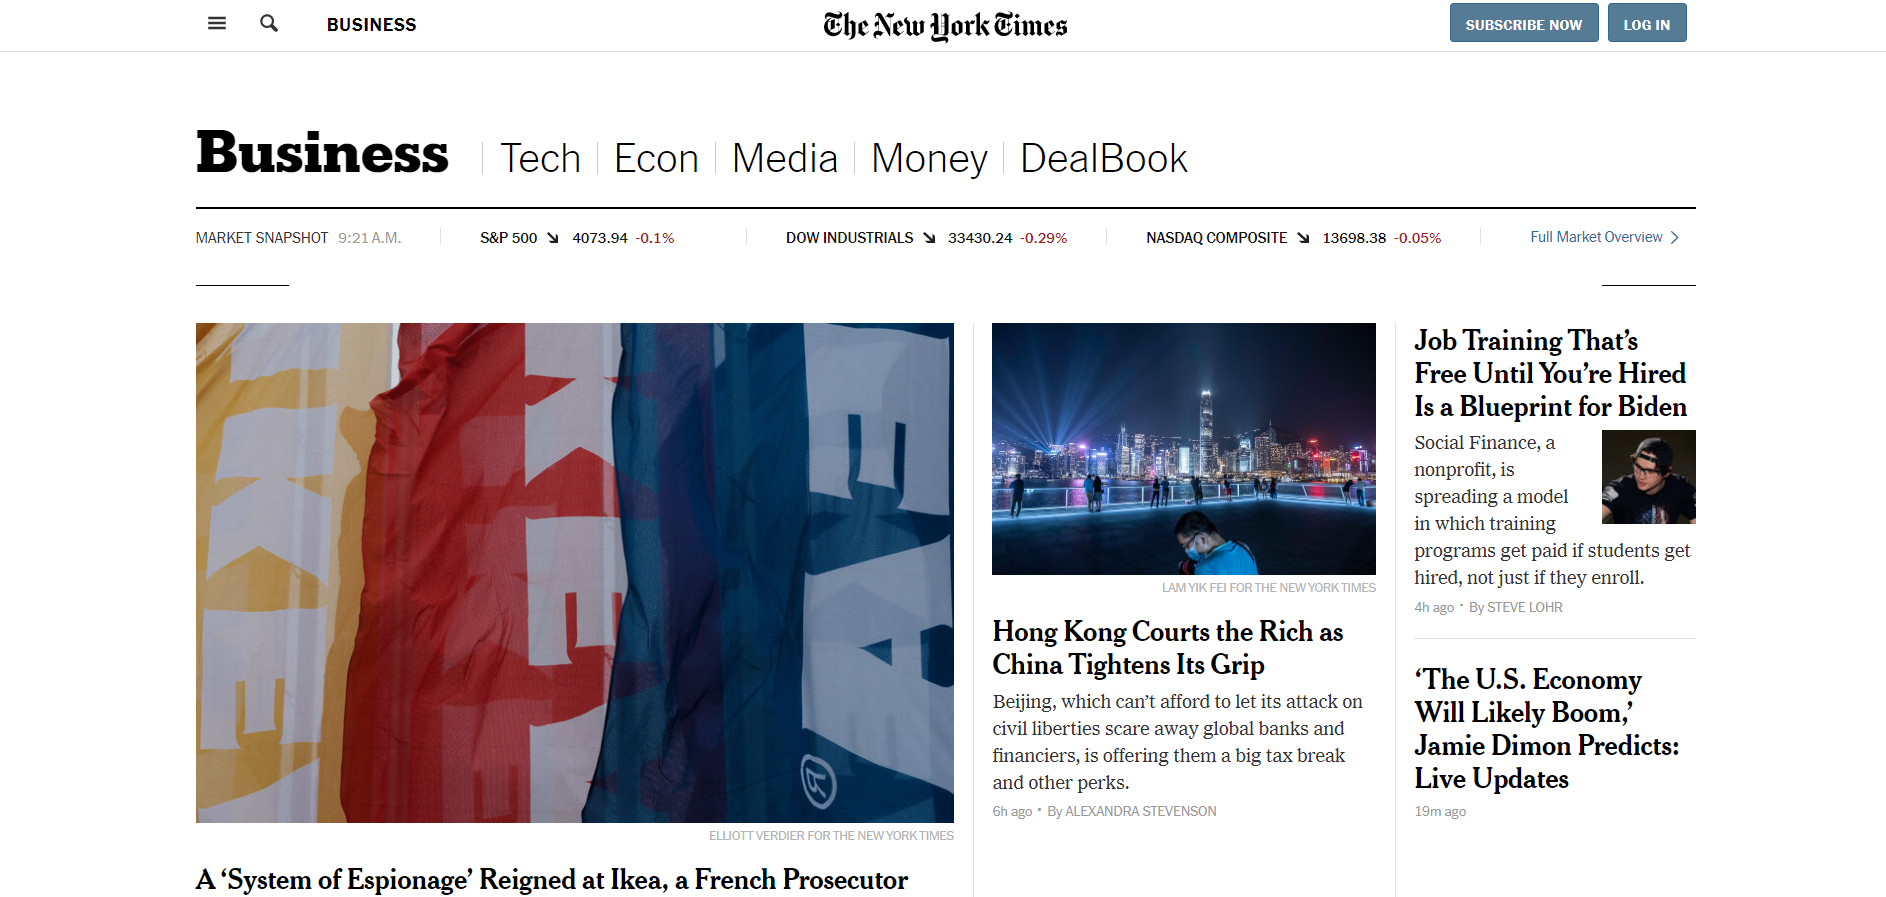
\includegraphics[height=5.2cm]{img/Other/responsive_desktop.png}}}%
	\quad
	\subfloat[Smartphone view]{\fbox{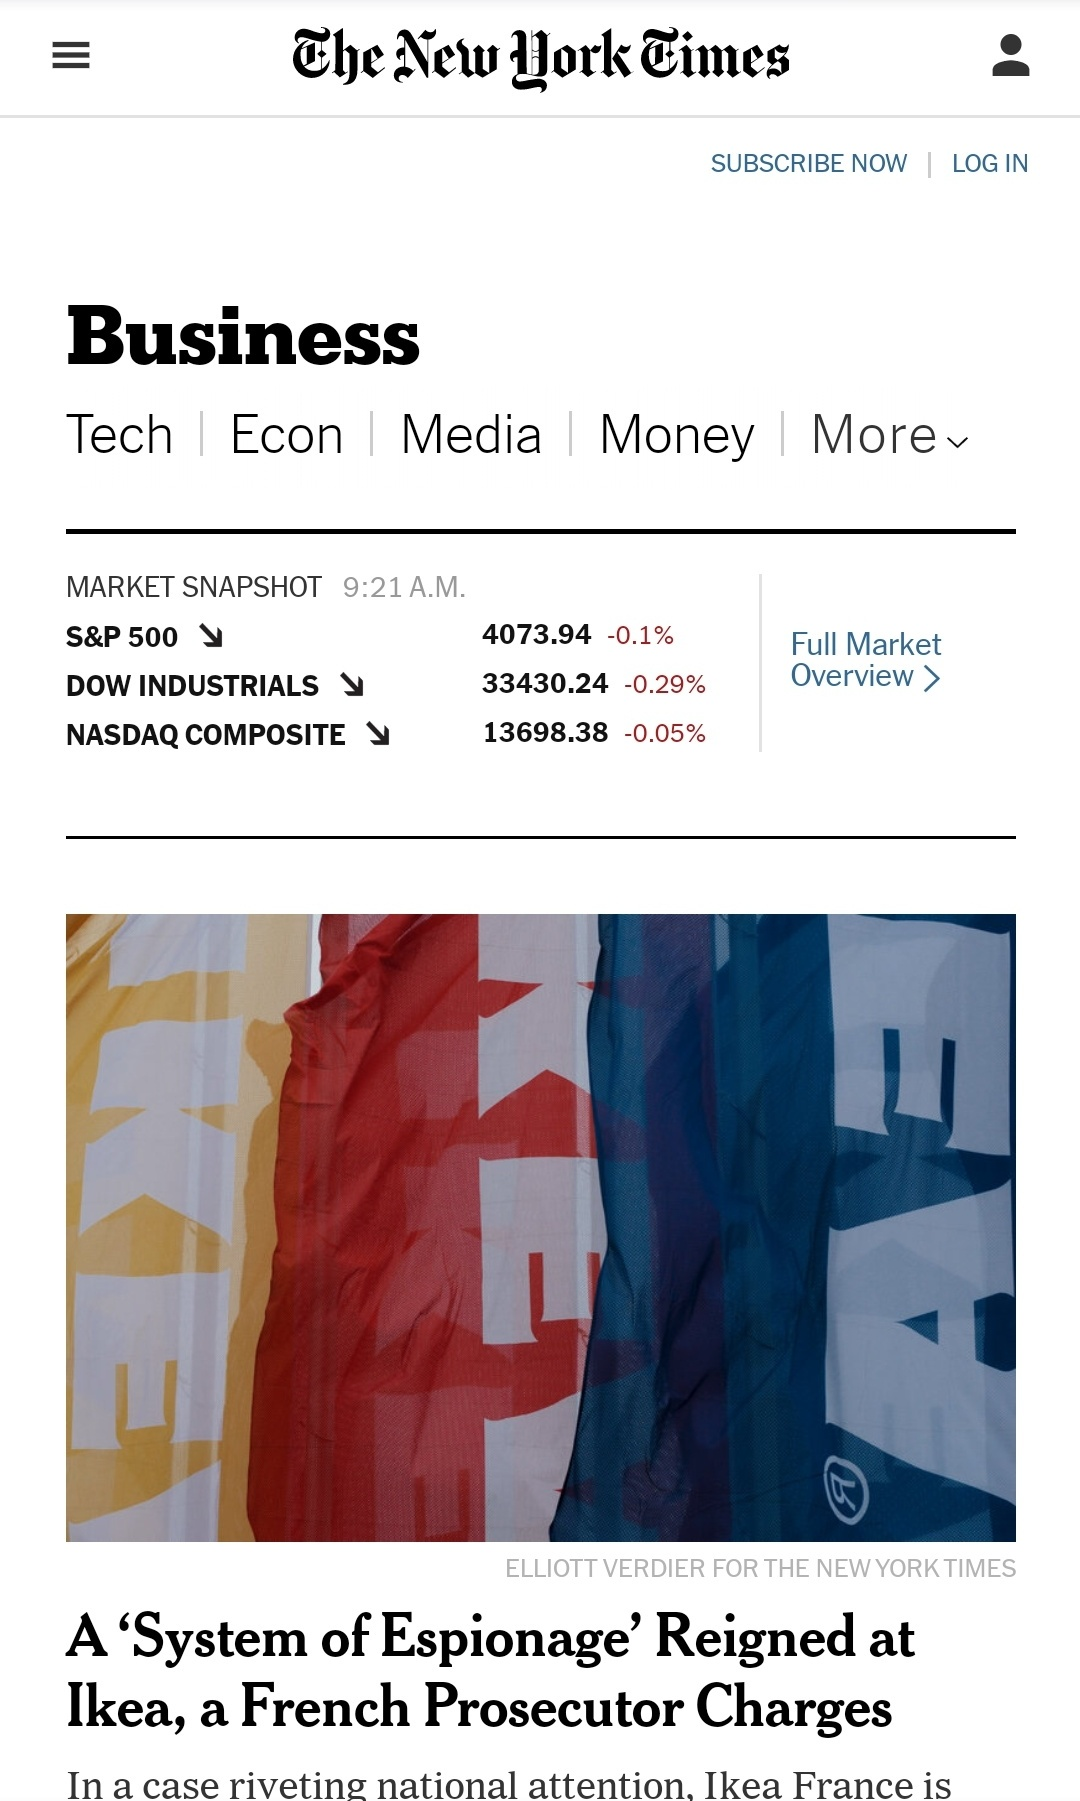
\includegraphics[height=5.2cm]{img/Other/responsive_mobile.jpg}}}%
	\caption{New York Times website responsiveness}%
	\label{fig:responsiveness}%
\end{figure}

\subsection{Native Mobile Applications}
A native application, or app, is a program developed to run on a specific type of mobile platform, developed using programming languages, application programming interfaces (APIs), and software development kits (SDKs) specific to that platform \cite{crossplatform_taxonomy, mobile_web_apps_2013}. A native app has full access to the device’s hardware and APIs, enabling the use of features such as the camera, storage, Bluetooth, and near-field communication (NFC).

This approach to mobile development results in apps that can only be run natively on one specific platform. This means that if an app is to be run on another platform, it needs to be remade with the tools and languages specific to the new platform. For example, if an Android application developed using the Java language is to be compatible with Apple devices using the iOS operating system, it needs to be recreated using the Swift programming language instead.

A native mobile application is distributed through a mobile storefront, also called an app store, which differs depending on the platform. The storefronts have policies and rules dictating what content is allowed on the store which developers must adhere to. Today, the most popular storefronts are  Google’s “Play Store” for Android devices and Apple’s “App Store” for iOS devices \cite{numofapps_in_stores}.

If an app is installed through one of these storefronts, updates to that app will be published and installed through that same storefront. Each update needs to be developed separately for each OS and published on its corresponding storefront, a process that might take different amounts of time depending on the storefronts’ policies. Maintaining consistency between versions running on different OS’s can therefore be difficult \cite{comp_mobile_apps_crossplatform}.

These qualities result in developing and maintaining native apps for multiple platforms at once being both time-consuming and costly \cite{mobile_web_apps_2013}.

In table \ref{tab:devstack}, the development stacks for Android and iOS are seen. Since the two platforms do not share programming languages, UI frameworks, or development tools, developing for both platforms is time consuming. An app developed to natively run on Android can not natively run on iOS, and vice versa.

\begin{table}[h]
\centering
\rowcolors{2}{black!10!white!100}{black!2!white!100}
\begin{tabular}{|l|l|l|}
\hline
\rowcolor[HTML]{656565}
\multicolumn{1}{|c|}{\cellcolor[HTML]{656565}} & {\color[HTML]{FFFFFF} Android} & {\color[HTML]{FFFFFF} iOS} \\ \hline
Programming language & Java, Kotlin & Objective-c, Swift \\
UI frameworks & Jetpack Compose, Android UI & UIKit, SwiftUI \\
Development Tools & Android Studio & Xcode, AppCode \\ \hline
\end{tabular}
\caption{Android an iOS development stack \cite{mobile_tech_stacks}}
\label{tab:devstack}
\end{table}

\subsection{Mobile Web Applications}
A mobile web app is a web application hosted on a remote server containing logic to serve content in a specific way to mobile devices \cite{crossplatform_2012, mobile_web_apps_2013}. Contrary to a native app, a web app is not installed on a mobile device but is instead accessed through a Uniform Resource Locator (URL) over the Hypertext Transfer Protocol (HTTP), and runs exclusively in the web browser \cite{crossplatform_taxonomy, crossplatform_2012}.

A web application, and by extension also a mobile web app, runs on a web server that handles all of the data processing and application logic. This leaves only the rendering of the user interface (UI) to the browser. Additionally, this also means no updates are required to be installed by the accessing device, all data resides on the webserver \cite{crossplatform_taxonomy, crossplatform_2012}

Since common web technologies like HTML5, CSS and JavaScript are used, the app is only developed once and can thereafter be accessed by any device using any sufficiently up-to-date browser, making it platform independent \cite{crossplatform_taxonomy}. Adversely, this dependence on browsers means that the app has many limitations such as  inability to access device hardware and software, inability to be published on a mobile storefront, high dependency on network connectivity, and potentially poor performance \cite{crossplatform_taxonomy, crossplatform_2012}

In Figure \ref{fig:webapp}, the architecture of a web app is seen. The browser fetches all necessary data from the web server that is hosting the application. Since a web app is built completely out of web technologies and runs exclusively in the browser, a user’s device does not need to install anything else.

\begin{figure}[h]%
	\centering
	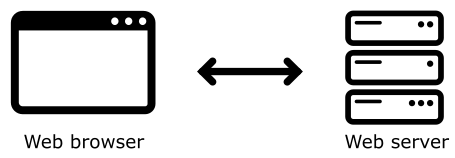
\includegraphics[height=3cm]{img/Other/struct_webapp.png}
	\caption{Web app architecture}%
	\label{fig:webapp}%
\end{figure}

\subsection{Hybrid Applications}
A hybrid app is essentially a mix of the native and web approaches to app development. The app is developed using the same tools as a web app, i.e. common web technologies, instead of native tools \cite{mobile_web_apps_2013}. A hybrid app executes inside a native container, or shell, and uses the device’s browser engine to render the common web elements inside a Web view \cite{crossplatform_2012}. This shell allows the hybrid app to function just like a native app would, allowing for the two approaches to be virtually indistinguishable for users. The shell also allows for the core of the app, such as the UI elements, to be reused across multiple platforms.

By making use of an abstraction layer, the web technologies that make up the app can access device hardware and software features through JavaScript APIs \cite{crossplatform_2012}. While a native app and a hybrid app have access to the same device features, this does not imply that the two are equivalent in performance. Since a hybrid app uses the browser engine, performance will naturally be lower than its native counterpart \cite{crossplatform_taxonomy, crossplatform_2012}.

A hybrid app can be distributed through platform-specific storefronts and cannot be used directly through the browser like a web app, a download of the full application is required to use it \cite{crossplatform_2012, mobile_web_apps_2013}. Just like a native app published on a storefront, updates are therefore also distributed through these same storefronts.

In Figure \ref{fig:hybridapp}, the architecture of a hybrid app is seen. The core app is a mobile web app wrapped in Web View. By the use of an abstraction layer, native functionality can be achieved.

\begin{figure}[h]%
	\centering
	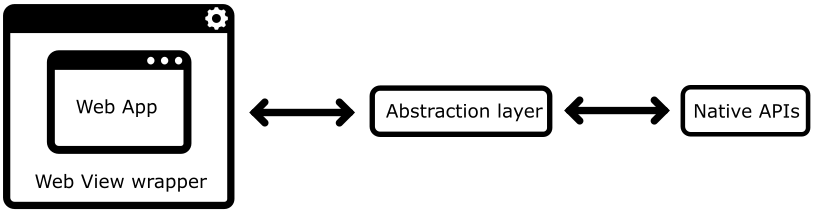
\includegraphics[height=3cm]{img/Other/struct_hybrid.png}
	\caption{Hybrid app architecture}%
	\label{fig:hybridapp}%
\end{figure}

\subsection{Progressive Web Applications}
While progressive web apps are not a new technology per se, they are mobile web apps that follow certain best practices and conventions. Since a PWA is built with the same technologies as normal mobile web apps they share many similarities;
\begin{itemize}
    \item a PWA can be accessed by any device with a sufficiently up-to-date web browser, making it platform-independent
    \item only one web app needs to be developed and maintained
    \item updates can be automatically applied without requiring additional downloads or installations
    \item no forced dependence on mobile storefronts
\end{itemize}

A PWA can be installed on a device and used like a native app, instead of being locked to a browser window like regular mobile web apps. When visiting a website, a prompt might pop up on the bottom of the screen containing the message “Add to home screen”. If the website is a PWA, clicking on it will start an installation procedure which finishes with an icon appearing on the device’s home screen. This icon will then be able to launch the installed app, instead of simply being a shortcut to a website.

PWAs were originally only installable from the browser, but today the three most popular mobile storefronts allow for the publishing of PWAs, including the Windows Store \cite{how_to_publish_pwa_in_stores}. This makes PWAs the most flexible in terms of usage options compared to native, hybrid, and mobile web apps.

To be considered a PWA, a web app must be served over HTTPS, have at least one service worker, and provide a web app manifest \cite{serviceworker_efficiency}. More on this in the following subSections.

\subsubsection{Web Workers \& Service Workers}
JavaScript is a single-threaded programming language, all instructions that are to be executed are placed on a stack and executed one by one \cite{mozilla_js}. Poor programming can therefore lead to greatly reduced performance in more complex applications.

A JavaScript web worker is an event-driven script that runs independently from the main document of a web page, effectively allowing for multiple threads of execution to be running concurrently. Web workers are intended to have a long lifespan and be used in lower numbers since they have both a high startup performance cost and a high memory cost while active. Web workers are therefore fit to handle complex tasks in the background to not slow down the main document thread that handles the normal UI functionality \cite{workers_html_spec}.

A service worker is a type of JavaScript web worker that can also act as a network proxy between the web page and the network. By sending the network requests to the worker the default network behavior can be overridden. One of the main benefits of this is the option to redirect network requests from the app to the cache instead of the server, effectively enabling offline access to the app. Additionally, the ability to deliver push notifications and sync data in the background while the app is not open is also enabled by the service worker \cite{service_workers_spec}.

\subsubsection{HTTPS}
On the internet, users with malicious intent can exploit essentially everything that gets sent over an unsecured connection, even data that might appear benign such as images or regular HTML. The Hypertext Transfer Protocol Secure, or just HTTPS for short, ensures that all requests to and from a website are encrypted and therefore secure \cite{why_https_matters}.

While protecting the integrity of a website’s users is important, HTTPS is also a requirement for many technologies that PWAs are using. Among others, service works and many APIs, such as the Geolocation API, are not usable without a secure HTTPS connection \cite{why_https_matters}.

\subsubsection{Web App Manifest}
A web app manifest is a JavaScript Object Notation (JSON) file including information about the app. The contents of the file are necessary for the app to function as a PWA since without it the web app would not be able to be downloaded and used as a native app.

The web app manifest includes information about the name, app icon, version, and background color, among other things. Data such as the app icon and name are especially important since without them the downloaded app would not be displayed like native apps on the device. Another important field is the URL which dictates what page the app should show when it is launched from the shortcut \cite{mozilla_webmanifest}.

A manifest file can have either the “.webmanifest” or “.json” file extensions and is linked in the head of HTML files in the web app in the same way that a CSS file would also be included \cite{mozilla_webmanifest}.

\subsubsection{PWA Architecture}
In Figure \ref{fig:pwaapp} the architecture of a PWA is seen. When the application makes a request to fetch some form of content from the remote web server, the service the request instead goes to the service worker. The service worker first checks whether the content exists in the cache; if so it is returned to the app and no network activity is needed. Only when the content has not been cached does the request go to the webserver.
\begin{figure}[h]%
	\centering
	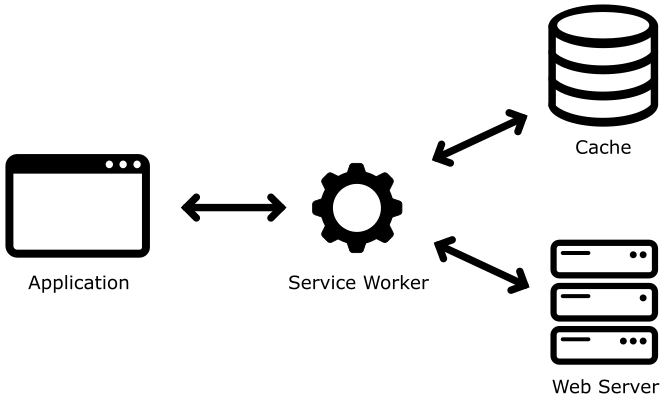
\includegraphics[height=6cm]{img/Other/struct_pwa.png}
	\caption{PWA architecture}%
	\label{fig:pwaapp}%
\end{figure}



\subsection{Mobile App Technologies - Feature Comparison}
Table X is a summary of what has been presented about the different mobile app and web development techniques in Sections 3.1 to 3.5. Sources \cite{mobile_web_apps_2013, dawning_of_pwa, pwa_in_modern_webdeb} were primarily used when deciding which rows were to be included in the table. Note that the column “MWA” refers to Mobile Web Apps.

The table is structured as a checklist to compare the features of each technique, with three possible checkmarks:
\begin{itemize}
    \item[] \cmark \quad indicates excellent support
    \item[] \textasciitilde \quad indicates partial support
    \item[] \xmark \quad indicates poor or no support
\end{itemize}

\begin{table}[h]
\centering
\rowcolors{2}{black!10!white!100}{black!2!white!100}
\begin{tabular}{|l|c|c|c|c|}
\hline
\rowcolor[HTML]{656565}
\multicolumn{1}{|c|}{\cellcolor[HTML]{656565}{\color[HTML]{FFFFFF} }} & \multicolumn{1}{c|}{\cellcolor[HTML]{656565}{\color[HTML]{FFFFFF} Native}} & \multicolumn{1}{c|}{\cellcolor[HTML]{656565}{\color[HTML]{FFFFFF} Hybrid}} & \multicolumn{1}{c|}{\cellcolor[HTML]{656565}{\color[HTML]{FFFFFF} MWA}} & \multicolumn{1}{c|}{\cellcolor[HTML]{656565}{\color[HTML]{FFFFFF} PWA}} \\ \hline
Installable & \cmark & \cmark & \xmark & \cmark \\
Offline access & \textasciitilde & \textasciitilde & \xmark & \cmark \\
Storefront distribution available & \cmark & \cmark & \xmark & \cmark \\
Mobile push notifications & \cmark & \cmark & \xmark & \cmark \\
Full platform API access & \cmark & \cmark & \xmark & \textasciitilde \\
Background sync & \cmark & \cmark & \textasciitilde & \cmark \\
Linkable, search indexable & \xmark & \xmark & \cmark & \cmark \\
No manual user updates & \xmark & \xmark & \cmark & \cmark \\
Easy to distribute & \textasciitilde & \textasciitilde & \cmark & \cmark \\
Desktop availability & \xmark & \xmark & \cmark & \cmark \\
Great performance & \cmark & \xmark & \xmark & \textasciitilde \\
Cross-platform & \xmark & \cmark & \cmark & \cmark \\
Low cross-platform dev cost & \xmark & \textasciitilde & \cmark & \cmark \\
\hline
\end{tabular}
\caption{Feature comparison of mobile app technologies}
\label{tab:mobilefeaturecomp}
\end{table}

\newpage

\section{Research Project}
This chapter contains detailed descriptions of all activities performed during the project both leading up to and during data collection.

When searching for grey literature on the subject, Google was the search engine of choice since it is currently the most widely used search engine \cite{search_engine_stats}. The search terms used during the literature study are seen in Table \ref{tab:searchterms}. Before entering any search terms in the search engine, the precautions seen in the following list were taken:

\begin{itemize}
    \item No Google account was signed in to avoid bias or optimizations.
    \item Only results from the past 2 years were shown to filter out outdated sources.
    \item Only results in English were shown.
    \item Location/region-specific search results were disabled.
\end{itemize}

\begin{table}[h]
\centering
\rowcolors{2}{black!10!white!100}{black!2!white!100}
\begin{tabular}{|c|l|}
\hline
\rowcolor[HTML]{656565}
\multicolumn{1}{|c|}{\cellcolor[HTML]{656565}{\color[HTML]{FFFFFF} Identifier}} & \multicolumn{1}{l|}{\cellcolor[HTML]{656565}{\color[HTML]{FFFFFF} Search query}} \\ \hline
ST1 & Progressive web application pros and cons \\
ST2 & PWA pros and cons \\
ST3 & PWA cons \\
\hline
\end{tabular}
\caption{Literature study search terms}
\label{tab:searchterms}
\end{table}

The final search term, ST3, proved to be the most effective at finding the desired information since ST1 and ST2 included a greater number of results that focused on the positive aspects and advantages. For this short literature study, the disadvantages of the technique were more relevant, since a greater quantity of the questions in the survey is to focus on drawbacks and desired changes from developers. Since many of the sources included only a small number of disadvantages, 15 sources were decided upon being a fitting sample size. If the number of disadvantages in each source was greater, a smaller number of sources would have been selected.

When searching for scientific sources, Google Scholar was used with the “Advanced search” feature. The search results were filtered to only be from 2019 - 2021, and to include at least one of the terms “PWA” or “Progressive web app”. Additional terms such as “features”, “comparison”, “vs native”, “disadvantages” and “evaluation” were also used to further narrow the searches. Even while using some of the additional terms, relevant sources were somewhat elusive. The 3 sources chosen for the study were sources \cite{dawning_of_pwa, pwa_in_modern_webdeb, pwa_unified}.

Once the material was read, many issues were identified. The issues were then grouped together based on what the perceived problem area of each issue was. These groups were then summarized into a small number of different concrete problem areas, which can be seen in Section 5.1. The problem areas that were only mentioned in a single source were omitted.

\subsection{Survey Design}
This Section details the creation of the survey questions. The questions are presented individually in Sections 4.2.2 and 4.2.3, but do not contain all of the options the participants have to choose from. The full questionnaires with all questions and options can be found in Appendix B and B.

\subsubsection{Survey Tool: Google Forms}
The surveys were created using the online survey tool Google Forms \cite{google_forms}. The choice of survey tool has a substantial impact on what type of questions can be asked, how the survey can be distributed, how the results are presented, and how the results can be exported. Google Forms was chosen due to its ease of use, aesthetics, and relatively strong feature set.

Google Forms allows for both open (qualitative) and closed (quantitative) questions, but a mix between the two is not possible. Qualitative questions were mainly preferred in this project since they allow for the participants to in more detail explain their thoughts and opinions. Due to this preference, there was a need to extend some of the quantitative questions to include the option for the participant to further clarify their opinion or thought processes. In Google Forms, quantitative questions that give “Yes/No/Maybe” answers can not be extended to instead be “Yes: explain/No: explain/Maybe: explain”. A separate follow-up question asking for further clarification is needed to be added instead. This solution works but results in the questions being asked in a slightly different way. For example, there is now a need to add follow-up questions such as “Please explain your reasoning behind your answer to the previous question”. Not a drawback that makes certain questions unaskable, but a drawback that results in a greater number of questions being asked.

\subsubsection{Developer Survey Questions}
The decision to split the surveys into distinct sections, or parts, was made before the questions were written. This was done both for the benefit of the project and the participants since the questions themselves become easier to create and answer if they are grouped together based on specific topics. The parts that were decided upon for the developer survey were the following 6:

\begin{enumerate}
    \item Personal Details
    \item Experience
    \item PWA
    \item Your Company \& Clients
    \item Mobile applications
    \item Final Thoughts
\end{enumerate}

The questions for the different Parts of the survey are shown and discussed in the coming paragraphs and tables, except for Part 5. This part does not include questions like the other parts. It is only included to allow for participants to add any comments, suggestions, and thoughts they might have.

The questions for Part 1 and Part 2 of the survey are shown in table \ref{tab:devq1} and table \ref{tab:devq2} respectively. The questions in these parts do not contribute directly to the answers for the research questions but do instead provide details about the demographic. All of these questions are quantitative to give a clear picture of the demographic without the need for deep analysis of qualitative answers. Note that in the table, “DSQ 1” should be read as “Developer survey, question 1” or something similar.

\begin{table}[h]
\centering
\rowcolors{2}{black!10!white!100}{black!2!white!100}
\begin{tabular}{|l|l|}
\hline
\rowcolor[HTML]{656565}
\multicolumn{1}{|c|}{\cellcolor[HTML]{656565}{\color[HTML]{FFFFFF} Number}} & \multicolumn{1}{l|}{\cellcolor[HTML]{656565}{\color[HTML]{FFFFFF} Question}} \\ \hline
DSQ 1 & In which country do you work? \\
DSQ 2 & Company name \\
DSQ 3 & What is your age? \\
\hline
\end{tabular}
\caption{Questions for dev Part 1: Personal Details}
\label{tab:devq1}
\end{table}

\begin{table}[h]
\centering
\rowcolors{2}{black!10!white!100}{black!2!white!100}
\begin{tabular}{|l|p{11cm}|}
\hline
\rowcolor[HTML]{656565}
\multicolumn{1}{|c|}{\cellcolor[HTML]{656565}{\color[HTML]{FFFFFF} Number}} & \multicolumn{1}{l|}{\cellcolor[HTML]{656565}{\color[HTML]{FFFFFF} Question}} \\ \hline
DSQ 4 & How many years have you worked as a developer? \\
DSQ 5 & What Best describes your current profession? \\
DSQ 6 & What type of applications have you previously developed or worked on? \\
DSQ 7 & Have you ever worked with any of the following cross-platform frameworks? \\
\hline
\end{tabular}
\caption{Questions for dev Part 2: Experience}
\label{tab:devq2}
\end{table}

The questions in Part 3 of the survey are shown in table \ref{tab:devq3} and all directly asking the developers about their opinion, experience, and knowledge of PWA. The questions primarily contribute to answering research questions 2, 3, and 4.

Question 8 is asked to gain more general knowledge about developers’ relation to PWA and to allow for more in-depth discussion, not to directly answer a research question.  This question also acts as a guide for how an individual participant’s answers should be evaluated. A developer with great knowledge of PWA should be able to provide more relevant answers than that of a developer with little or no knowledge.

Questions 10 to 13 contribute to the answer to research question 2 (if developers experience the same issues as the literature describes). Questions 10 and 11 are qualitative and allow the participant to describe their development preferences, which might include mentioning specific issues. Questions 12 and 13 are instead qualitative and directly ask about specific issues identified in the conducted literature study.

Questions 9 to 11 and 14 to 16 all contribute to answering research question 3 (developers’ opinions of PWA today and of its future). These questions are a mix of quantitative and qualitative to give a wider variety of information that allows for greater opportunities for discussion and analysis.

\begin{table}[h]
\centering
\rowcolors{2}{black!10!white!100}{black!2!white!100}
\begin{tabular}{|l|p{11cm}|}
\hline
\rowcolor[HTML]{656565}
\multicolumn{1}{|c|}{\cellcolor[HTML]{656565}{\color[HTML]{FFFFFF} Number}} & \multicolumn{1}{l|}{\cellcolor[HTML]{656565}{\color[HTML]{FFFFFF} Question}} \\ \hline
DSQ 8 & How good is your knowledge of PWA? \\
DSQ 9 & Would you consider developing a PWA in the future? \\
DSQ 10 & Is there anything that makes you prefer other cross-platform solutions over PWA? \\
DSQ 11 & Is there anything that makes you prefer developing natively over PWA? \\
DSQ 12 & Have you ever encountered any of the following problems with PWA? \\
DSQ 13 & When was the last time you encountered any of the problems above? \\
DSQ 14 & What is your opinion on PWA as a development technique today? \\
DSQ 15 & How much do you agree with this statement: "PWA is the future of mobile app development" \\
DSQ 16 & If you disagree, how do you think PWAs need to change before the statement becomes true? \\
\hline
\end{tabular}
\caption{Questions for dev Part 3: PWA}
\label{tab:devq3}
\end{table}

\newpage Part 4 of the survey asks questions about the developers’ companies and their clients, which is seen in table \ref{tab:devq4}. Questions 17 and 18 are purely quantitative and contribute to research question 4 (if clients influence the decision of PWA versus other solutions). Question 19 on the other hand does not answer any research questions but is yet another additional point of discussion.

\begin{table}[ht]
\centering
\rowcolors{2}{black!10!white!100}{black!2!white!100}
\begin{tabular}{|l|l|}
\hline
\rowcolor[HTML]{656565}
\multicolumn{1}{|c|}{\cellcolor[HTML]{656565}{\color[HTML]{FFFFFF} Number}} & \multicolumn{1}{l|}{\cellcolor[HTML]{656565}{\color[HTML]{FFFFFF} Question}} \\ \hline
DSQ 17 & Has a client ever asked for a PWA? \\
DSQ 18 & Have you ever proposed PWA as a solution to a client? \\
DSQ 19 & What type of apps does your company offer? \\
\hline
\end{tabular}
\caption{Questions for dev Part 4: Your company \& clients}
\label{tab:devq4}
\end{table}

Finally, Part 5 of the survey asks the participant to rank the importance of several characteristics and features of mobile apps and can be seen in table \ref{tab:devq5}. This question is quantitative and answers research question 1 (if PWA fulfills the most important characteristics of mobile apps).

\begin{table}[h!]
\centering
\rowcolors{2}{black!10!white!100}{black!2!white!100}
\begin{tabular}{|l|l|}
\hline
\rowcolor[HTML]{656565}
\multicolumn{1}{|c|}{\cellcolor[HTML]{656565}{\color[HTML]{FFFFFF} Number}} & \multicolumn{1}{l|}{\cellcolor[HTML]{656565}{\color[HTML]{FFFFFF} Question}} \\ \hline
DSQ 20 & Please rank the importance of the following qualities of mobile apps  \\
\hline
\end{tabular}
\caption{Questions for dev Part 5: Mobile apps}
\label{tab:devq5}
\end{table}

\subsubsection{Education Survey Questions}
The survey was divided into 5 different parts, much like the developer survey. The parts that were decided upon for the education survey were the following 4:

\begin{itemize}
    \item Personal details \& experience
    \item Mobile applications
    \item PWA
    \item Final Thoughts
\end{itemize}

Just like for the developer survey, the final part is not for asking questions but is instead for feedback. Of note is that the education survey is completely separate from the developer survey, which is why some questions appear duplicated.

The questions for Part 1 of the survey are shown in table \ref{tab:eduq1}. Just like for the developer survey, the first part is only to give a better understanding of the participants. Note that in the table, “ESQ 1” should be read as “Education survey, question 1” or something similar. Additional note about ESQ 1 is that it is redundant since all participants in the education survey are from Sweden. This question is here because the survey constructed before the decision to limit the survey to only Swedish education was made.

\begin{table}[ht]
\centering
\rowcolors{2}{black!10!white!100}{black!2!white!100}
\begin{tabular}{|l|l|}
\hline
\rowcolor[HTML]{656565}
\multicolumn{1}{|c|}{\cellcolor[HTML]{656565}{\color[HTML]{FFFFFF} Number}} & \multicolumn{1}{l|}{\cellcolor[HTML]{656565}{\color[HTML]{FFFFFF} Question}} \\ \hline
ESQ 1 & In which country do you work? \\
ESQ 2 & Where do you work? \\
ESQ 3 & What is your age? \\
ESQ 4 & In which of the following subjects do you teach? \\
ESQ 5 & How long have you been teaching in these subjects? \\
\hline
\end{tabular}
\caption{Questions for edu Part 1: Personal details \& experience}
\label{tab:eduq1}
\end{table}

The questions for Part 2 of the survey are seen in table \ref{tab:eduq2} and are about mobile applications. Questions 6 to 8 are purely quantitative and all contribute to answering research question 6 (if PWA is covered in higher education courses about app development).

Question 9 is the same as the last question in the developer survey; it asks the participant to rank the importance of mobile app characteristics. This question can contribute to answering research question 1 and its results might be extra interesting if it differs significantly from the rankings that developers gave.
\newpage

\begin{table}[ht]
\centering
\rowcolors{2}{black!10!white!100}{black!2!white!100}
\begin{tabular}{|l|p{11cm}|}
\hline
\rowcolor[HTML]{656565}
\multicolumn{1}{|c|}{\cellcolor[HTML]{656565}{\color[HTML]{FFFFFF} Number}} & \multicolumn{1}{l|}{\cellcolor[HTML]{656565}{\color[HTML]{FFFFFF} Question}} \\ \hline
ESQ 6 & What type of applications do your courses cover? \\
ESQ 7 & If your courses do not cover cross-platform apps, do you think it should be covered in the future? \\
ESQ 8 & If your courses do cover cross-platform apps, does it cover any of the following frameworks? \\
ESQ 9 & Please rank the importance of the following features and qualities of mobile apps \\
\hline
\end{tabular}
\caption{Questions for edu Part 2: Mobile applications}
\label{tab:eduq2}
\end{table}

Part 3 of the survey is about PWAs and all its questions can be seen in table \ref{tab:eduq3}. Since only one of the research questions are specifically about the education sector, all of the questions in this part aims to answer research question 6.

\begin{table}[ht]
\centering
\rowcolors{2}{black!10!white!100}{black!2!white!100}
\begin{tabular}{|l|l|}
\hline
\rowcolor[HTML]{656565}
\multicolumn{1}{|c|}{\cellcolor[HTML]{656565}{\color[HTML]{FFFFFF} Number}} & \multicolumn{1}{l|}{\cellcolor[HTML]{656565}{\color[HTML]{FFFFFF} Question}} \\ \hline
ESQ 10 & How good is your knowledge of PWA? \\
ESQ 11 & Is PWA mentioned in the required literature in any of your courses? \\
ESQ 12 & Is PWA part of the curriculum in any of your courses? \\
ESQ 13 & If not, please give a short explanation \\
ESQ 14 & Has it ever been requested that PWA be included in the curriculum? \\
ESQ 15 & If yes, from whom? \\
ESQ 16 & Do you think PWA should be included in the curriculum? \\
\hline
\end{tabular}
\caption{Questions for edu Part 3: PWA}
\label{tab:eduq3}
\end{table}

\subsection{Survey Questions Relation to Research Questions}
Table \ref{tab:sq_relation_to_rq} depicts how the survey questions contribute to the answer of the research questions. Questions 1-8 and 19 in the developer survey as well as questions 1-5 in the education survey do not appear in the table. The omitted questions do not directly contribute to the answer of any of the research questions but do instead help to understand the demographic that was covered by the survey. These questions also open up for further possible analysis and conclusion drawing at the end of the project.

\begin{table}[h]
\centering
\rowcolors{2}{black!10!white!100}{black!2!white!100}
\begin{tabular}{|l|c|c|c|c|c|c|}
\hline
\rowcolor[HTML]{656565}
\multicolumn{1}{|c|}{\cellcolor[HTML]{656565}{\color[HTML]{FFFFFF} }} & \multicolumn{1}{c|}{\cellcolor[HTML]{656565}{\color[HTML]{FFFFFF} RQ 1}} & \multicolumn{1}{c|}{\cellcolor[HTML]{656565}{\color[HTML]{FFFFFF} RQ 2}} & \multicolumn{1}{c|}{\cellcolor[HTML]{656565}{\color[HTML]{FFFFFF} RQ 3}} & \multicolumn{1}{c|}{\cellcolor[HTML]{656565}{\color[HTML]{FFFFFF} RQ 4}} & \multicolumn{1}{c|}{\cellcolor[HTML]{656565}{\color[HTML]{FFFFFF} RQ 5}} & \multicolumn{1}{c|}{\cellcolor[HTML]{656565}{\color[HTML]{FFFFFF} RQ 6}} \\ \hline
DSQ 9 &  &  & \xmark &  &  &  \\
DSQ 10 &  & \xmark & \xmark &  &  &  \\
DSQ 11 &  & \xmark & \xmark & \xmark &  &  \\
DSQ 12-13 &  & \xmark &  &  &  &  \\
DSQ 14 &  &  & \xmark &  &  &  \\
DSQ 15 &  &  & \xmark &  &  &  \\
DSQ 16 &  &  & \xmark & \xmark &  &  \\
DSQ 17 &  &  &  &  & \xmark &  \\
DSQ 18 &  &  &  &  & \xmark &  \\
DSQ 20 & \xmark &  &  &  &  &  \\
ESQ 6-8 &  &  &  &  &  & \xmark \\
ESQ 9 & \xmark &  &  &  &  &  \\
ESQ 10-16 &  &  &  &  &  & \xmark \\
\hline
\end{tabular}
\caption{Feature comparison of mobile app technologies}
\label{tab:sq_relation_to_rq}
\end{table}

\newpage
\subsection{Survey Participant Selection}
This Section details the process of selecting participants.

\subsubsection{Participating Countries - Developer Survey}
From the following four countries, the participants for the survey were selected.
\begin{itemize}
    \item Sweden
    \item Poland
    \item USA
    \item India
\end{itemize}

These countries are located on three different continents; Europe, North America, and South Asia. They were chosen to represent as broad of a demographic as possible to avoid an overwhelming bias in favor of one particular country or community. Since both of the surveys are completely in English, an additional consideration when selecting countries was that the general knowledge of the English language of the population needed to be high.

Poland was not originally a part of the investigation. During the selection process it was discovered that several companies have offices in both Sweden and Poland. The apparent prevalence of Polish developers resulted in a slight expansion of the scope of the investigation to further include this demographic.

\subsubsection{The Clutch.co Directory}
For finding companies to contact, the application developer directory offered by Clutch \cite{clutch} was chosen as the source. This directory offers the option to filter companies based on which countries they have offices in via the “Location” input. Other useful information can also be found such as what “Service focus” a company has and in which country their headquarters are located. Service focus refers to services such as “Social media marketing” or “Web development” and is expressed as percentages of their overall business.

This directory offers an easier way to search than if a traditional search engine such as Google or Bing was used since irrelevant results and advertisements are not shown. There are two major drawbacks with Clutch that can affect the results of the investigation. Firstly, the companies shown first by default are labeled as “Sponsors” of the platform. This problem can be rectified by changing the sorting option to for instance be “Number of reviews” or “Company name”. Secondly, showing up in the Clutch directory requires a manual application process. The number of companies that have been through this process varies greatly between countries which might mean that many potential candidates for participation are not considered at all. If the investigation had a broader scope, this issue might have been deemed big enough to include companies from other sources as well.

\subsubsection{Selection Process - Developer Survey}
The following requirements need to be fulfilled before a company could be selected to be a participant in the survey.

\begin{itemize}
    \item The company must have specified that at least 15\% of their service focus is “Mobile App Development”
    \item The company must have an office in the country in question, preferably its headquarters
    \item The company must have a functioning website. Sites that did not load or were automatically blocked as being “unsafe” by Google Chrome were not further pursued
    \item The company must \textbf{not} have specified that their business is strictly in Native development
    \item The company must have either a contact form or a specified contact email that is \textbf{not} exclusively for sales or business inquiries.
\end{itemize}

The directory is paginated with 40 companies per page. Sweden had only about 2 pages on compared to the around 100 pages each for the other three countries. Due to the much smaller number of companies, requirement 1 was deemed not necessary to fulfill for a Swedish company to be considered for participation.

If a company fulfilled all requirements the following details were saved in a document:

\begin{itemize}
    \item Company name
    \item Contact email address or contact form link
    \item Website link
    \item Any additional notes to keep in mind when contacting them
    \item Have they been contacted?
\end{itemize}

The goal during this process was to save the information about 35 companies from each country for a grand total of 140 different companies. About 20 of the companies were not contacted on the basis of the email address not being reachable or the contact form not being functional.

\subsubsection{Selection Process - Education Survey}
A list of higher educational institutes in Sweden was used to find people to contact for the education survey \cite{higher_edu_sweden}. Only the schools listed under the headings "Universitet" and "Högskolor" were included in the search.

At the website of each school, the main information that was searched for was either a list of courses or a search function for courses. Filtering options to only show courses related to computer science or IT were used whenever possible. A course believed to be fit for further investigation had its syllabus read through. If the syllabus mentioned that the course was about web or mobile app development it was considered for the survey. Some courses that were only about information or interface design were not included.

If a contact person was explicitly given on the course page they were directly contacted about the survey. If no contact person was given an email asking for the contact information for the courses was sent to the school instead. Out of the total 10 courses found fit for the survey, only the contact person for one of them was not able to be reached.


\newpage
\section{Results}
This chapter presents the results from the short literature study and the survey answers.

\subsection{Literature Study}
The literature study was split into two parts, with the first part examining 15 sources of grey literature and the second part examining 3 sources of scientific literature. The problem areas identified in all the literature were organized and grouped together based on what the underlying issue was. These groups, or more accurately categories, can be seen in the table \ref{tab:lit_study_result}. Additionally, the table includes how many times these issues were mentioned in both the grey literature and the scientific literature, expressed both as a raw number and as a percentage of the total.

\begin{table}[h]
\centering
\rowcolors{2}{black!10!white!100}{black!2!white!100}
\begin{tabular}{|c|p{5.5cm}|c|c|c|}
\hline
\rowcolor[HTML]{656565}
\multicolumn{1}{|p{1.5cm}|}{\cellcolor[HTML]{656565}{\color[HTML]{FFFFFF} Category}} & {\cellcolor[HTML]{656565}{\color[HTML]{FFFFFF} Issue/problem area}} & \multicolumn{1}{p{1.6cm}|}{\cellcolor[HTML]{656565}{\color[HTML]{FFFFFF} \quad Grey mentions}} & \multicolumn{1}{p{1.65cm}|}{\cellcolor[HTML]{656565}{\color[HTML]{FFFFFF} Scientific mentions}} & \multicolumn{1}{p{1.6cm}|}{\cellcolor[HTML]{656565}{\color[HTML]{FFFFFF} \quad Total}} \\ \hline
CAT 1 & Hardware access limitations & 11 & 3 & 78\% (14)  \\
CAT 2 & Additional limitations on iOS & 10 & 2 & 67\% (12)  \\
CAT 3 & Visibility/marketplace presence & 9 & 1 & 56\% (10)  \\
CAT 4 & Software limitations & 7 & 1 & 44\% (8)  \\
CAT 5 & Higher battery consumption & 7 & 0 & 39\% (7)  \\
CAT 6 & Legacy device/browser support & 4 & 3 & 39\% (7)  \\
CAT 7 & Cross login/Inter-app communication & 2 & 0 & 11\% (2)  \\

\hline
\end{tabular}
\caption{Feature comparison of mobile app technologies}
\label{tab:lit_study_result}
\end{table}

Categories 1-3 were all mentioned in above 50\% of the sources, categories 4-6 were mentioned in around 40\% of sources and finally, category 7 was mentioned in only 11\% of sources.

A difference between most of the grey literature and the scientific literature is the type of content they typically included and how it was presented. Most grey sources used bullet lists for presenting the many advantages and disadvantages at once to allow for an easy overview. The scientific sources tended to include a smaller number of issues that were discussed in much greater detail.

\subsection{Developer Survey}
This Section presents the results from the survey aimed at application developers. The survey reached out to 122 different companies that offer app or website development to their clients. The contacted companies were from Sweden, USA, India, and Poland, with about an even split between the four countries. From the 122 companies contacted, 16 different developers participated in the survey.

\subsubsection{Part 1 - Personal Details}
This part of the survey was not aimed at directly answering any of the research questions. The questions asked in this part were for the purpose of enabling more in-depth analysis and discussion and to help identify potential biases.

\begin{figure}[ht!]
    \centering
    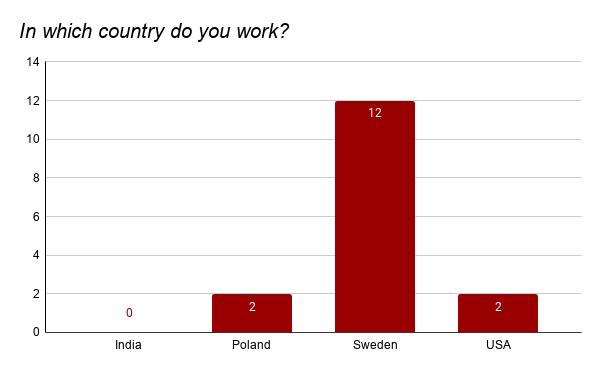
\includegraphics[width=10cm]{img/Results/dsq1.png}
    \caption{Answers for DSQ 1}
    \label{fig:res_devq1}
\end{figure}

The first question asked respondents about which country they work in, results seen in Figure \ref{fig:res_devq1}. Most participants (12/16) were from Sweden, while Poland and the USA both had two participants. None of the Indian companies participated in the survey.

DSQ 2 is not shown in a diagram like all the other survey questions. DSQ 2 was an optional question that asked respondents to specify which company they work for. For the sake of the privacy of the respondents this information is omitted from the report. Most respondents (10/16) did not answer this question, but of the ones who did 4 were from the same company.

\begin{figure}[ht!]
    \centering
    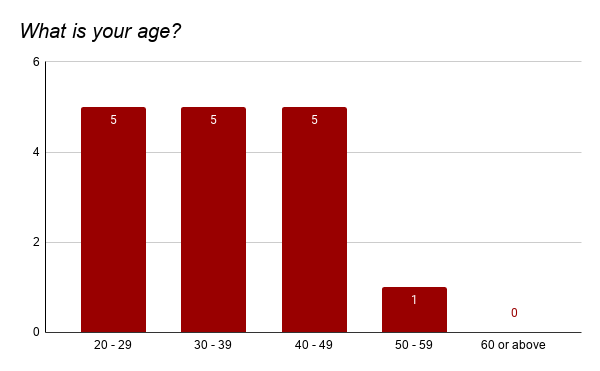
\includegraphics[width=10cm]{img/Results/dsq3.png}
    \caption{Answers for DSQ 3}
    \label{fig:res_devq3}
\end{figure}

DSQ 3 asked for which age group the participants belonged to, results seens in Figure \ref{fig:res_devq3}. Only one respondent was between the age of 50 to 59 years old. five respondents each belonged to the age groups 20-29, 30-39, and 40-49.

\subsubsection{Part 2 - Experience}
Much like Part 1 of the survey, Part 2 also asked questions for the purpose of allowing for greater discussion. The questions in Part 2 of the survey helped paint the picture of how experienced respondents were with native and cross-platform development.

\begin{figure}[ht!]
    \centering
    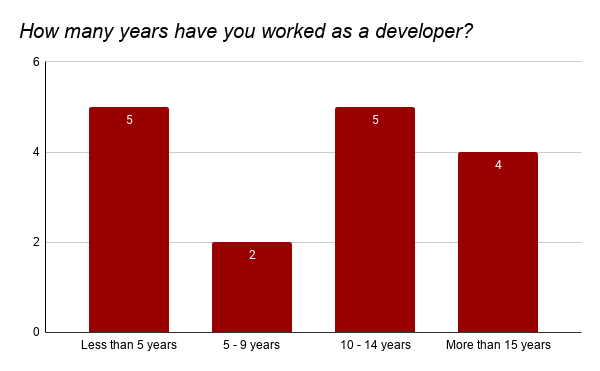
\includegraphics[width=10cm]{img/Results/dsq4.png}
    \caption{Answers for DSQ 4}
    \label{fig:res_devq4}
\end{figure}

DSQ 4 asked how many years of experience as a developer the respondents had, results seen in Figure \ref{fig:res_devq4}. The main purpose of this question was to see if developers of different experience levels have different preferences and opinions of cross-platform development and PWA. Two respondents had between 5 and 9 years of experience while 4 respondents had more than 15 years of experience. The remaining 10 respondents were evenly split between 10 to 14 years of experience and less than five years of experience.

\begin{figure}[ht!]
    \centering
    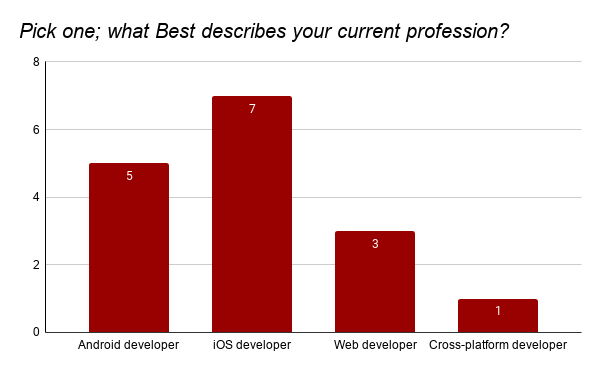
\includegraphics[width=10cm]{img/Results/dsq5.png}
    \caption{Answers for DSQ 5}
    \label{fig:res_devq5}
\end{figure}

DSQ 5 asked what best describes the current profession of the respondent, results seen in Figure \ref{fig:res_devq5}. The purpose of this questions was to was to see how for instance Android developers' opinions of PWA differs from that of iOS developers. Five respondents were Android developers, seven were iOS developers, three were web developers, and only once was a cross-platform developer.

\begin{figure}[ht!]
    \centering
    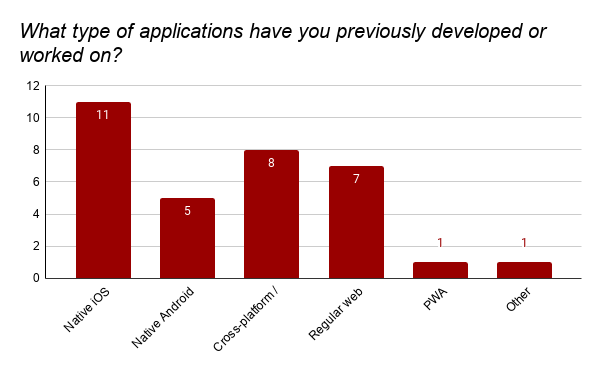
\includegraphics[width=10cm]{img/Results/dsq6.png}
    \caption{Answers for DSQ 6}
    \label{fig:res_devq6}
\end{figure}

DSQ 6 asked respondents what type of applications they have previously worked on, results seen in Figure \ref{fig:res_devq6}. Much like DSQ 4 and 5, this question was asked to see how developers experience might influence their answers to later questions. Most respondents (11/16) had worked on iOS apps before, while only some respondents (5/16) had worked on Android apps before. Eight respondents had worked on cross-platform apps and seven had worked on regular web apps. Only one respondent had worked on a PWA before. One respondent added that they had also worked on applications not included in the list of options which was software for embedded Linux systems.

\begin{figure}[ht!]
    \centering
    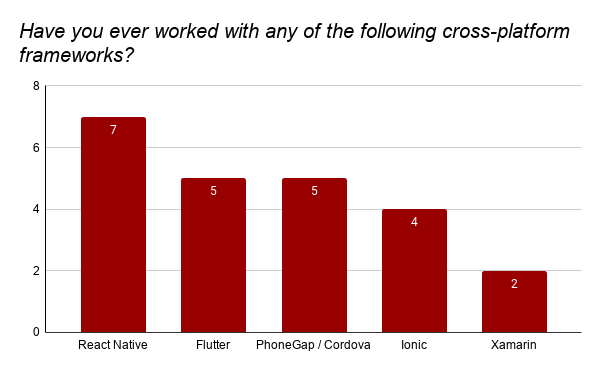
\includegraphics[width=10cm]{img/Results/dsq7.png}
    \caption{Answers for DSQ 7}
    \label{fig:res_devq7}
\end{figure}

DSQ 7 asked respondents what frameworks for cross-platform development they have used in the past, results seen in Figure \ref{fig:res_devq7}. This question was asked to gauge the general popularity of different frameworks. A similar question was also asked in the education survey to see what frameworks are included in curricula, so education versus real-world popularity can be compared. React Native was the most popular of the frameworks at seven responses. Flutter, PhoneGap or Cordova, and Ionic were the second most popular at five, five, and 4 responses respectively. Xamarin was the least used framework at only two responses.

\subsubsection{Part 3 - PWA}
This part of the survey had the goal of answering research questions 2, 3, and 4. The questions were a mix of quantitative and qualitative and were quite mixed in what they were asking. All questions in this part were about PWA.

\begin{figure}[ht!]
    \centering
    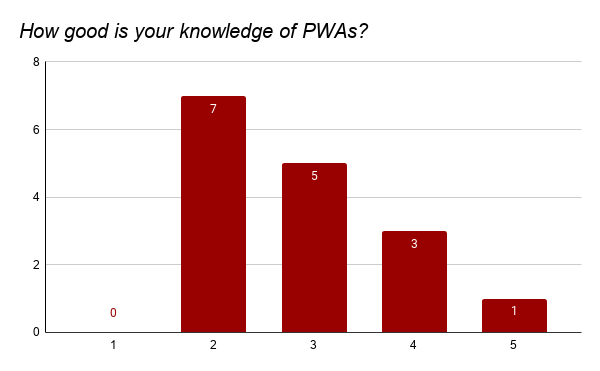
\includegraphics[width=10cm]{img/Results/dsq8.png}
    \caption{Answers for DSQ 8}
    \label{fig:res_devq8}
\end{figure}

DSQ 8 asked the respondents about their perceived level of knowledge of PWA, results seen in Figure \ref{fig:res_devq8}. The answers were given on a scale of one to five, with one being "None" and five being "Very good". All respondents had at least some knowledge of PWA, since 0/16 responded that their knowledge was a 0/5. A majority of the respondents said their knowledge of PWA was a either a 2/5 (7/16 respondents) or 3/5 (5/16 respondents), which would correspond to "low" and "ok" respectively. Three responded with a 4/5 while only one responded with a 5/5, scores that corresponds to "good" and "very good" level of knowledge respectively.

\begin{figure}[ht!]
    \centering
    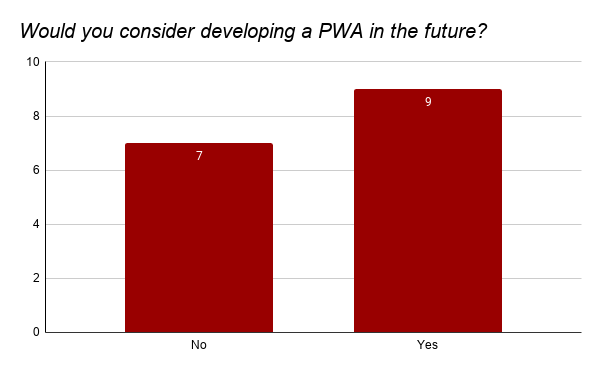
\includegraphics[width=10cm]{img/Results/dsq9.png}
    \caption{Answers for DSQ 9}
    \label{fig:res_devq9}
\end{figure}

DSQ 9 asked if the respondents would consider developing a PWA in the future, results seen in Figure \ref{fig:res_devq9}. The question received a very split result: a small majority (9/16) responded with "Yes" while a small minority (7/16) responded with a "No". Research question 3 is about what developers think of PWA and its future. RSQ 9 does not directly ask their opinion on PWA, but the answers the respondents give can still be used to answer the research question.

\begin{figure}[ht!]
    \centering
    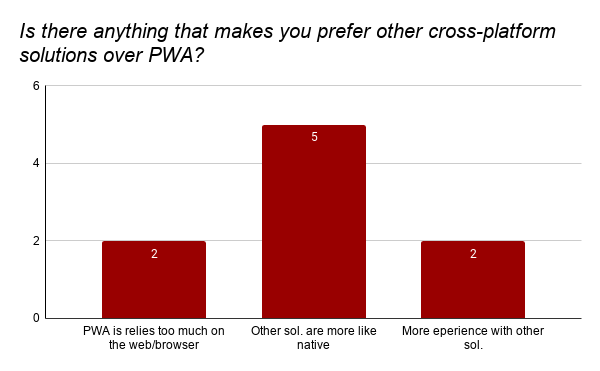
\includegraphics[width=10cm]{img/Results/dsq10.png}
    \caption{Summary of answers for DSQ 10}
    \label{fig:res_devq10}
\end{figure}

\newpage
DSQ 10 asked if there is anything that makes the respondents prefer development with other cross-platform solutions, a summary of the results are seen in Figure \ref{fig:res_devq10}. The answers were split according to what the issues brought up were related to. This question was optional and received responses from 8 respondents, with one response fitting into two categories at once. A majority of respondents (5/8) mentioned that a cross-platform solution that is "more like native" was preferable. Examples include mentioning that React Native uses "native components" and that other solutions "take less effort to integrate with the native platform". Two responses mentioned that PWA relied too much on the browser, with one respondent saying that this made PWA "unreliable". Two responses mentioned that their preference was  based on them having more experience with other solutions. This question helps answer both research question 2 and 3 since some responses mentioned opinions of PWA (RQ 3) and some mentioned problems with PWA (RQ 2).

\begin{figure}[ht!]
    \centering
    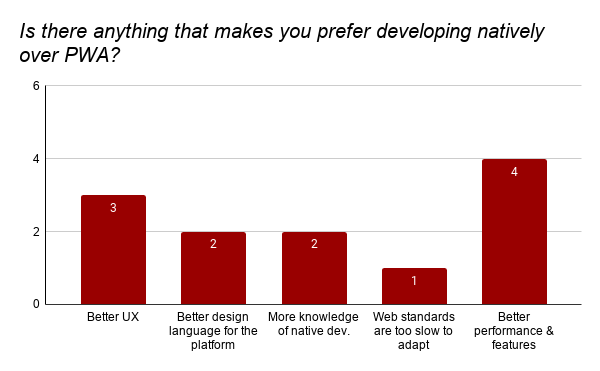
\includegraphics[width=10cm]{img/Results/dsq11.png}
    \caption{Answers for DSQ 11}
    \label{fig:res_devq11}
\end{figure}

DSQ 11 asked if there is anything that makes the respondents prefer development of native apps to that of PWA, a summary of the results are seen in Figure \ref{fig:res_devq11}. The answers were split according to what the issues brought up were related to. This question was optional and received responses from 11 respondents, with several responses fitting into two or more categories at once. Four responses mentioned that native has either better performance or access to better features. Three responses mentioned that native offers a better user experience (UX) in general. Two responses mentioned that the design language with native is better fit for the target platform. Two responses mentioned that they prefer native development since they have more experience with it. One response mentioned that web standards "can take ages to get adopted by browser vendors" while for native the access to new features is much quicker. This question helps answer research question 2, 3, and 4 since the responses include current problems with PWA (RQ 2 \& RQ 3) and what is holding it back from being more widely used (RQ 4).

\begin{figure}[ht!]
    \centering
    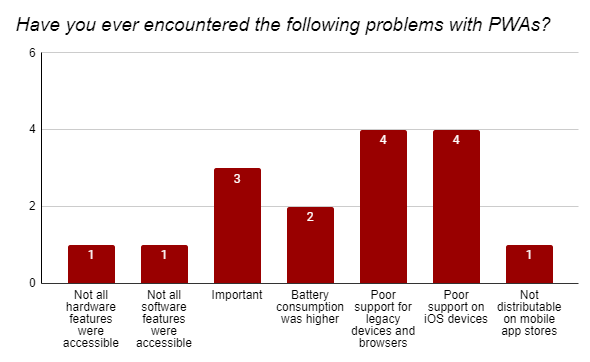
\includegraphics[width=10cm]{img/Results/dsq12.png}
    \caption{Answers for DSQ 12}
    \label{fig:res_devq12}
\end{figure}

DSQ 12 asked if the respondents had experienced any of a specific set of problems with PWA, answers seen in Figure \ref{fig:res_devq12}. Respondents could select multiple options. "Poor support on iOS" and "Not distributable on app stores" were each selected four times. "Battery consumption was higher" was selected three times. "Poor support for legacy devices" was selected two times. Being selected one time each was hardware and software access was limited. One respondent gave an original answer that was the a PWA "Doesn't feel at home on the phone". This question directly answers research question 2.

\begin{figure}[ht!]
    \centering
    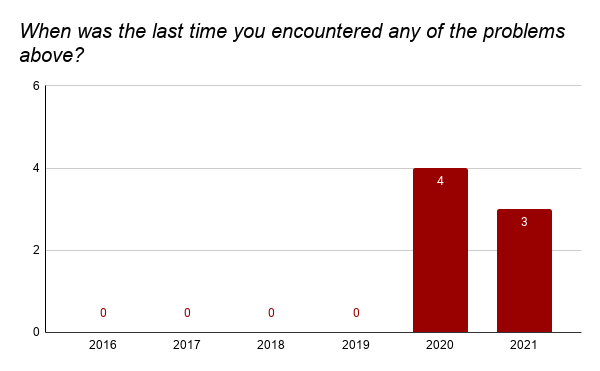
\includegraphics[width=10cm]{img/Results/dsq13.png}
    \caption{Answers for DSQ 13}
    \label{fig:res_devq13}
\end{figure}

DSQ 13 was a follow-up to DSQ 12 and asked when the last time any of the mentioned problems was encountered, results seen in Figure \ref{fig:res_devq13}. None of the respondents answered 2016, 2017, 2018, or 2019. Four of the respondents answered 2020 and three answered 2021.

\begin{figure}[ht!]
    \centering
    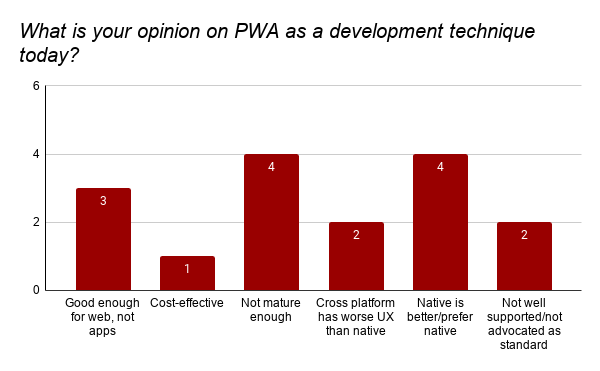
\includegraphics[width=10cm]{img/Results/dsq14.png}
    \caption{Summary of answers for DSQ 14}
    \label{fig:res_devq14}
\end{figure}

\newpage
DSQ 14 asked respondents of their opinion on PWA today, a summary of the results are seen in Figure \ref{fig:res_devq14}. Four respondents mentioned that they liked native better or that native development is better. Four respondents mentioned that the main problem with PWA was the it is not mature enough yet. Three respondents said that PWA is good enough for the web, but native development is better for apps.

\begin{figure}[ht!]
    \centering
    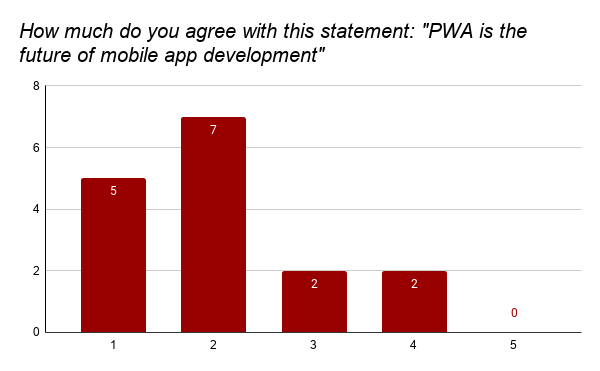
\includegraphics[width=10cm]{img/Results/dsq15.png}
    \caption{Answers for DSQ 15}
    \label{fig:res_devq15}
\end{figure}

DSQ 15 asked respondents to to rate their agreement with the statement that "PWA is the future of mobile development", results seen in Figure \ref{fig:res_devq15}. The answers were given on a scale of one to five, with one being "Strongly disagree" and five being "Strongly agree". A vast majority answered either 1 (5/16) or (7/16), meaning that disagreed with the statement. The options 3 and 4 were each chosen two times while the option 5 was not chosen by any respondents.

\begin{figure}[ht!]
    \centering
    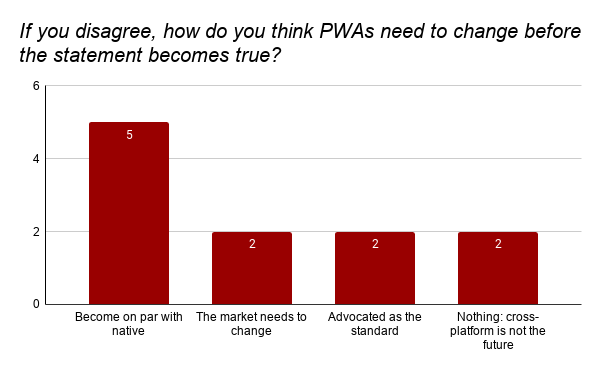
\includegraphics[width=10cm]{img/Results/dsq16.png}
    \caption{Summary of answers for DSQ 16}
    \label{fig:res_devq16}
\end{figure}

\newpage
DSQ 16 was a follow-up question to DSQ 15, asking respondents that disagreed with the statement in DSQ 15 to try and give an answer as to what is needed to change for the statement to become true, a summary of the results are seen in Figure \ref{fig:res_devq16}. Five respondents said that PWA needs to become at least on par with native in terms of for instance device API access. Two respondents pondered that maybe it is the market that needs to change to fit PWA instead of the other way around, while two respondents stated that since PWA is cross-platform, it cannot be the future. Two respondents talked about how PWA needs to be the standard on a platform, or at least advocated by Apple or Google. DSQ 15 and DSQ 16 together help answer research question 3, while DSQ 16 additionally help answer research question 4.

\subsubsection{Part 4 - Your Company \& Clients}
This part of the survey only asked a small number of question about the developers' employing companies and their clients. These questions together help answer research question 5, if clients influence the decision of using PWA or not.

\begin{figure}[ht!]
    \centering
    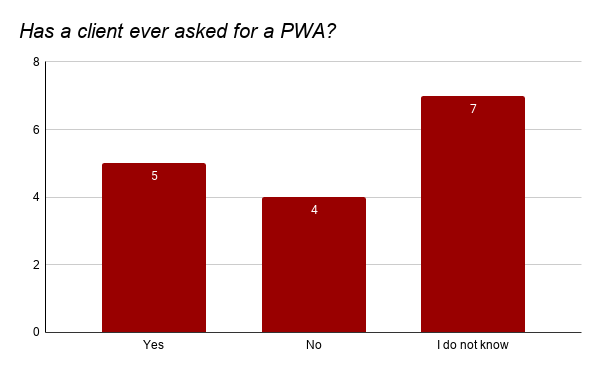
\includegraphics[width=10cm]{img/Results/dsq17.png}
    \caption{Answers for DSQ 17}
    \label{fig:res_devq17}
\end{figure}

DSQ 17 asked if a client ever requested a PWA, results seen in Figure \ref{fig:res_devq17}. Seven respondents answered that they do not know if a client has request PWA. Five respondents answered "Yes" and four answered "No", a very evenly split result.

\begin{figure}[ht!]
    \centering
    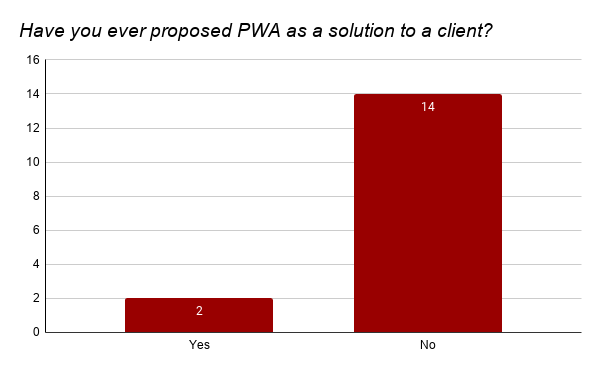
\includegraphics[width=10cm]{img/Results/dsq18.png}
    \caption{Answers for DSQ 18}
    \label{fig:res_devq18}
\end{figure}

DSQ 18 asked if the respondent had ever proposer PWA to a client, results seen in Figure \ref{fig:res_devq18}. An overwhelming majority of respondents (14/16) answered that they had not proposed PWA as a solution to a client while only two respondent that they had proposed it.

\begin{figure}[ht!]
    \centering
    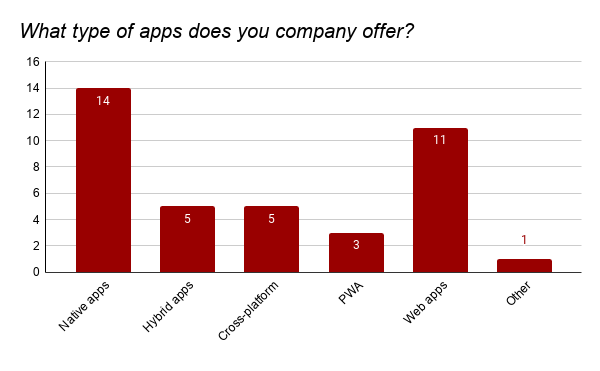
\includegraphics[width=10cm]{img/Results/dsq19.png}
    \caption{Answers for DSQ 19}
    \label{fig:res_devq19}
\end{figure}

DSQ 19 asked what types of applications the respondents' employing companies offered to clients, results seen in Figure \ref{fig:res_devq19}. This question was mainly asked to see if the respondents' experience correlates with what the company offers.

\subsubsection{Part 5 - Mobile applications}
This part of the survey contained only one question about how important certain aspects of mobile apps are according to developers. The question contains 9 sub-questions, one for each of the aspects/features that was to be ranked. This result is only presented in table \ref{tab:devq20} and will not be further described in this Chapter. Individual diagrams for each of the sub-questions can be seen in Appendix C.

One respondent added as a comment that two additional things that could have been asked in this question were "Native controls" and "Be a priority for the platform vendor to support". There was only one respondent that mentioned these two issues.

% Change table styling to make table fit horizontally
\setlength{\parindent}{0pt}
\setlength{\arrayrulewidth}{0.4mm}
\setlength{\tabcolsep}{4pt}
\renewcommand{\arraystretch}{1.5}

\begin{table}[h]
    \centering
    \rowcolors{2}{black!10!white!100}{black!2!white!100}
    \begin{tabular}{|p{3cm}|c|c|c|c|c|c|}
      \hline
      \rowcolor[HTML]{656565}  & \multicolumn{1}{p{1.7cm}|}{\textcolor{white}{Not at all important}}  & \multicolumn{1}{p{1.6cm}|}{\textcolor{white}{Slightly \shortstack important}}  &  \multicolumn{1}{p{1.7cm}|}{\textcolor{white}{Important}} & \multicolumn{1}{p{1.7cm}|}{\textcolor{white}{Fairly \shortstack important }}  & \multicolumn{1}{p{1.6cm}|}{\textcolor{white}{Very \shortstack important}}  & \multicolumn{1}{p{1.4cm}|}{\textcolor{white}{No opinion}} \\
      \hline
      Available on app stores & 0  & 0 & 1 & 7 & 8 & 0 \\
      \hline
      Installable (app store or web download)   & 1  & 0  & 1  & 6  & 8  & 0\\
      \hline
       Push notifications  &  0 & 1  & 0  &  2 &  13 &0 \\
      \hline
       Background sync   &  0 &  2 & 1  &  4 & 9  & 0\\
      \hline
       High  performance  &  0 &  0 &  0 & 7  & 9  & 0\\
      \hline
       Low battery  usage  & 0  & 0  & 2  & 5  &  9 & 0\\
      \hline
       Usable  while  offline &  0 &  5 & 3  &  3 &  5 & 0\\
      \hline
       Cross-platform  &  5 & 3  &  2 & 5  &  1 & 0\\
      \hline
       Discoverable from web-search  &  4 & 4  &  6 & 0  &  2 & 0\\
      \hline
    \end{tabular}
    \caption{Answers for DSQ 20}
    \label{tab:devq20}
\end{table}

\subsection{Education Survey}
The education survey reached out to nine different contact persons for courses in web or app development. The courses were taught in different institutes of higher education in Sweden. Out of the total of nine contacted persons, two participated in the survey.



\subsubsection{Part 1 - Personal Details}
This part of the survey was not aimed at directly answering any of the research questions, just like the first part of the Developer survey. The questions asked in this part were for the purpose of enabling more in-depth analysis and discussion and to help identify potential biases. Although since the number of responses was so low, this is not really possible in this case.

\begin{figure}[ht!]
    \centering
    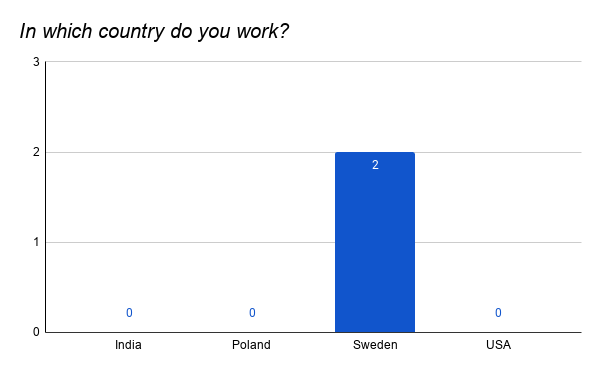
\includegraphics[width=10cm]{img/Results/esq1.png}
    \caption{Answers for ESQ 1}
    \label{fig:res_eduq1}
\end{figure}
\newpage
ESQ 1 asked the respondents to answer which country they work in, results seen in Figure \ref{fig:res_eduq1}. Both respondents were from Sweden.

ESQ 2 was optional and asked respondents which institute of higher education they worked in. The results of this question is not shown to protect the privacy of the respondents.

\begin{figure}[ht!]
    \centering
    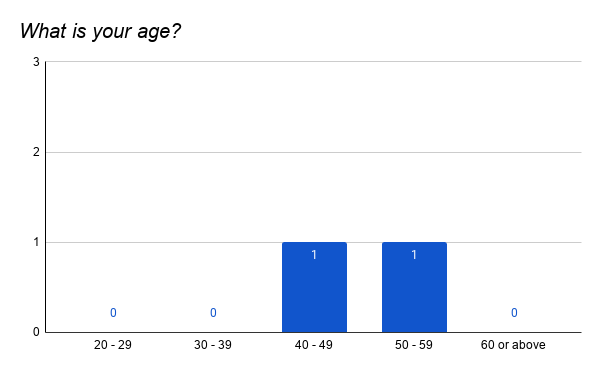
\includegraphics[width=10cm]{img/Results/esq3.png}
    \caption{Answers for ESQ 3}
    \label{fig:res_eduq3}
\end{figure}

ESQ 3 asked respondents which age group they belonged to, results seen in Figure \ref{fig:res_eduq3}. One respondent was between 40-49 years old while the other was between 50-59 years old.
\newpage

\begin{figure}[ht!]
    \centering
    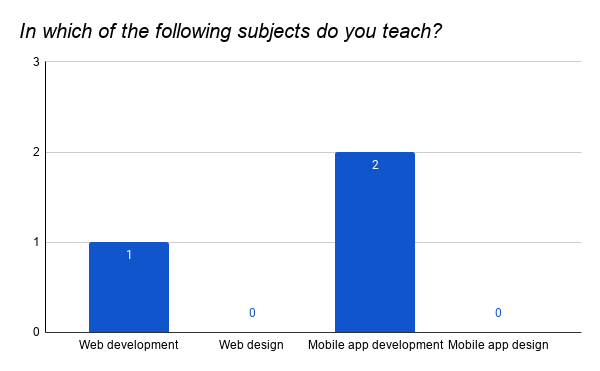
\includegraphics[width=10cm]{img/Results/esq4.png}
    \caption{Answers for ESQ 4}
    \label{fig:res_eduq4}
\end{figure}

ESQ 4 asked respondents what type of courses they teach, results seen in Figure \ref{fig:res_eduq4}. Both respondents teach in "Mobile app development" courses, and one respondent also teach in "Web development" courses.

\begin{figure}[ht!]
    \centering
    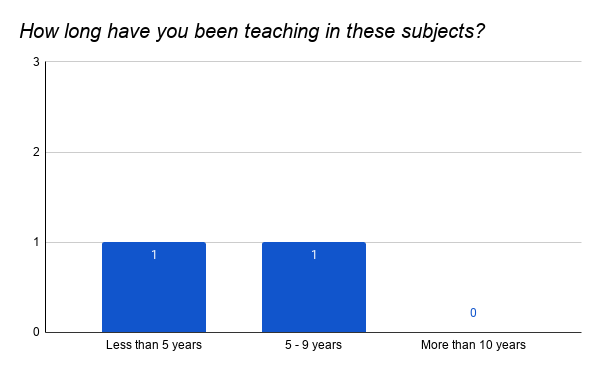
\includegraphics[width=10cm]{img/Results/esq5.png}
    \caption{Answers for ESQ 5}
    \label{fig:res_eduq5}
\end{figure}

ESQ 5 asked respondents for how long they had been teaching the subjects specific in ESQ 4, results seen in Figure \ref{fig:res_eduq5}. One respondent answered that they had been teaching the subjects for less than 5 years while the other answered 5-9 years.

\subsubsection{Part 2 - Mobile Applications}
This part of the survey asked questions about PWA, cross-platform in general, and the importance of mobile app qualities/features. These questions were asked so the answers could be directly compared to the answers given by developers.

\begin{figure}[ht!]
    \centering
    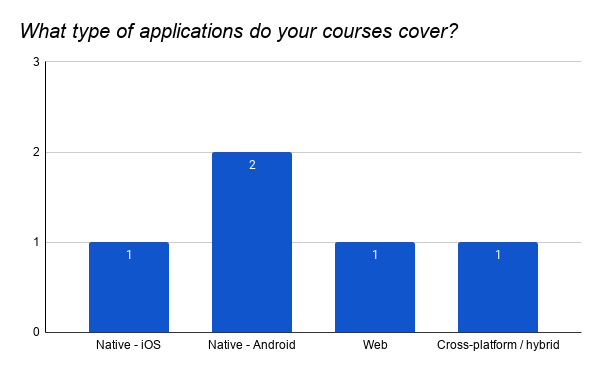
\includegraphics[width=10cm]{img/Results/esq6.png}
    \caption{Answers for ESQ 6}
    \label{fig:res_eduq6}
\end{figure}

\newpage
ESQ 6 asked respondents what type of applications their courses covered, results seen in Figure \ref{fig:res_eduq6}. Both respondents had courses in native android development. Native iOS, Web, and cross-platform/hybrid apps were covered in courses by one respondent. This question was asked to help answer research question 6 which is about the state of PWA coverage in higher education.

\begin{figure}[ht!]
    \centering
    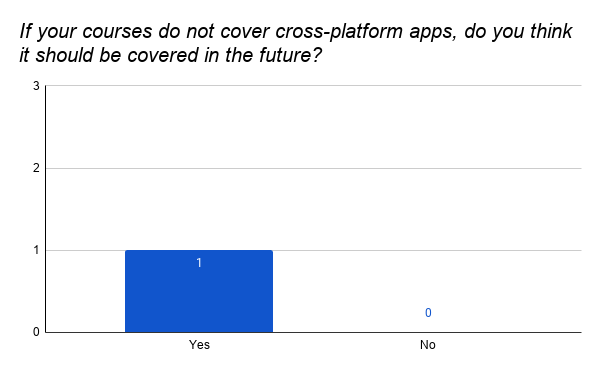
\includegraphics[width=10cm]{img/Results/esq7.png}
    \caption{Answers for ESQ 7}
    \label{fig:res_eduq7}
\end{figure}

ESQ 7 was a follow-up question to ESQ 6 and it asked respondents whose courses do not cover cross-platform if they think cross-platform development should be covered, results seen in Figure \ref{fig:res_eduq7}. The respondent answered that Yes, they do think cross-platform should be covered. This question was asked in conjunction with ESQ 6 to help answer research question 6.

\begin{figure}[ht!]
    \centering
    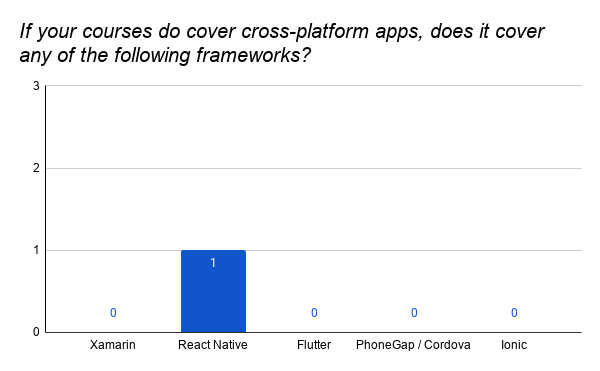
\includegraphics[width=10cm]{img/Results/esq8.png}
    \caption{Answers for ESQ 8}
    \label{fig:res_eduq8}
\end{figure}

\newpage
ESQ 8 was a follow-up question to ESQ 6 and it asked respondents whose courses do cover cross-platform what type of frameworks they cover, results seen in Figure \ref{fig:res_eduq8}. The respondent answered that the framework "React Native" was covered in their courses. This question was asked in conjunction with ESQ 6 to help answer research question 6.

\begin{table}[h]
    \centering
    \rowcolors{2}{black!10!white!100}{black!2!white!100}
    \begin{tabular}{|p{3cm}|c|c|c|c|c|c|}
      \hline
      \rowcolor[HTML]{656565}  & \multicolumn{1}{p{1.7cm}|}{\textcolor{white}{Not at all important}}  & \multicolumn{1}{p{1.6cm}|}{\textcolor{white}{Slightly \shortstack important}}  &  \multicolumn{1}{p{1.7cm}|}{\textcolor{white}{Important}} & \multicolumn{1}{p{1.7cm}|}{\textcolor{white}{Fairly \shortstack important }}  & \multicolumn{1}{p{1.6cm}|}{\textcolor{white}{Very \shortstack important}}  & \multicolumn{1}{p{1.4cm}|}{\textcolor{white}{No opinion}} \\
      \hline
      Available on app stores & 0  & 1 & 1 & 0 & 0 & 0 \\
      \hline
      Installable (app store or web download)   & 0  & 0  & 0  & 0  & 2  & 0\\
      \hline
       Push notifications  &  0 & 0  & 0  &  2 &  0 &0 \\
      \hline
       Background sync   &  0 &  2 & 0  &  0 & 0  & 0\\
      \hline
       High  performance  &  0 &  0 &  0 & 1  & 1  & 0\\
      \hline
       Low battery  usage  & 0  & 1  & 1  & 0  &  0 & 0\\
      \hline
       Usable  while  offline &  0 &  1 & 0  &  0 &  1 & 0\\
      \hline
       Cross-platform  &  0 & 0  &  0 & 2  &  0 & 0\\
      \hline
       Discoverable from web-search  &  0 & 1  &  0 & 0  &  1 & 0\\
      \hline
    \end{tabular}
    \caption{Answers for ESQ 9}
    \label{tab:eduq9}
\end{table}

\newpage
ESQ 9 is a duplicate of DSQ 20, meaning that the question contains 9 sub-questions, one for each of the aspects/features of mobile apps that was to be ranked. Just like for DSQ 20, this result is only presented in table \ref{tab:eduq9} and will not be further described in this Chapter. Individual diagrams for each of the sub-questions can be seen in Appendix D.

\begin{figure}[ht!]
    \centering
    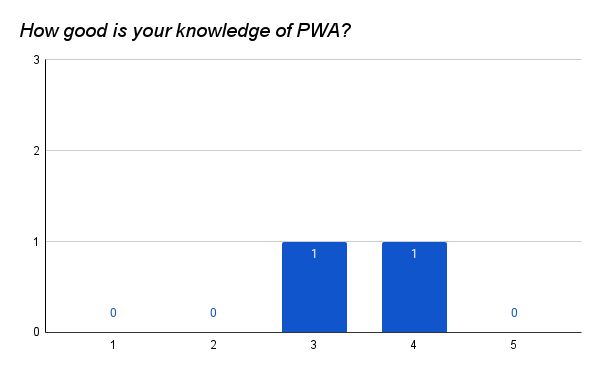
\includegraphics[width=10cm]{img/Results/esq10.png}
    \caption{Answers for ESQ 10}
    \label{fig:res_eduq10}
\end{figure}

\subsubsection{Part 3 - PWA}
This part of the survey had the goal of answering research question 6. All questions in this part were about PWA.

ESQ 10 is a duplicate of DSQ 8 and asked the respondents about their perceived level of knowledge of PWA, results seen in Figure \ref{fig:res_devq10}. The answers were given on a scale of one to five, with one being "None" and five being "Very good". One respondent answered 3/5 and one respondent answered 4/5, which corresponds to an "ok" and "good" level of knowledge respectively.

\begin{figure}[ht!]
    \centering
    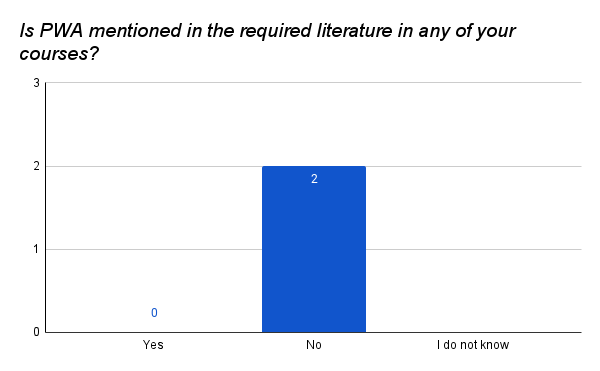
\includegraphics[width=10cm]{img/Results/esq11.png}
    \caption{Answers for ESQ 11}
    \label{fig:res_eduq11}
\end{figure}

ESQ 11 asked respondents whether or not PWA was covered by the required literature of their courses, results seen in Figure \ref{fig:res_eduq11}. Both respondents answered "No" to the question.

\begin{figure}[ht!]
    \centering
    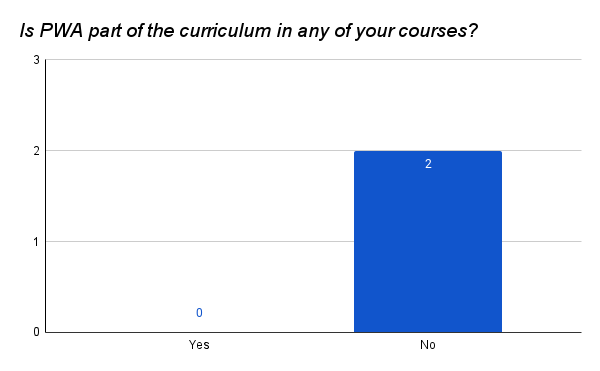
\includegraphics[width=10cm]{img/Results/esq12.png}
    \caption{Answers for ESQ 12}
    \label{fig:res_eduq12}
\end{figure}

ESQ 12 asked respondents whether or not PWA was mentioned in the curriculum of their courses, results seen in Figure \ref{fig:res_eduq12}. Both respondents answered "No" to the question.

\begin{figure}[ht!]
    \centering
    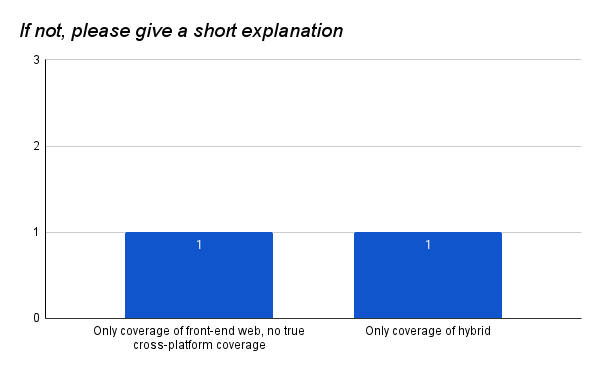
\includegraphics[width=10cm]{img/Results/esq13.png}
    \caption{Summary of answers for ESQ 13}
    \label{fig:res_eduq13}
\end{figure}

\newpage ESQ 13 was a follow-up to ESQ 12 and asked respondents to elaborate on why PWA was not covered in their courses, results seen in Figure \ref{fig:res_eduq13}. One respondent answered that the only cross-platform they covered was front-end web with JavaScript frameworks, but that no "true" cross-platform development was covered. One respondent answered that the only cross-platform apps covered by their courses were hybrid apps with the "React Native" framework.

\begin{figure}[ht!]
    \centering
    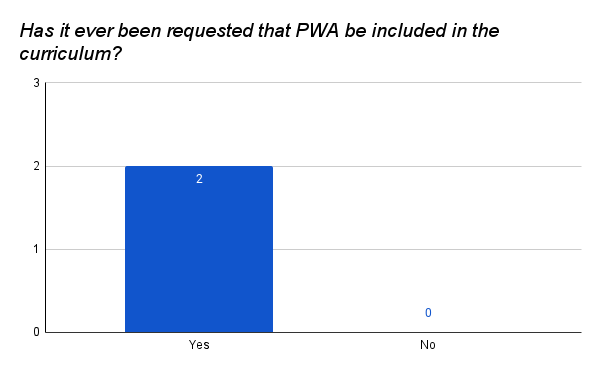
\includegraphics[width=10cm]{img/Results/esq14.png}
    \caption{Answers for ESQ 14}
    \label{fig:res_eduq14}
\end{figure}

ESQ 14 asked respondents whether or not it had ever been request that PWA was added to their courses, results seen in Figure \ref{fig:res_eduq14}. Both respondents answered "Yes" to the question.

\begin{figure}[ht!]
    \centering
    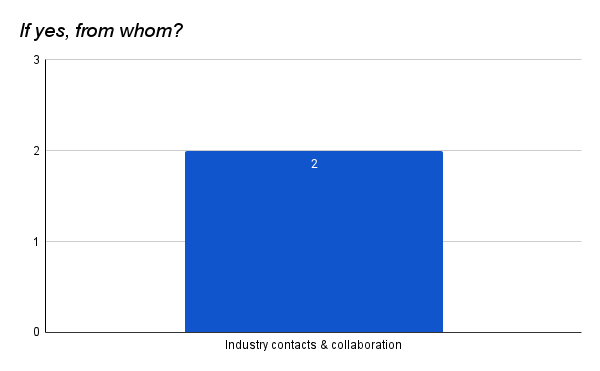
\includegraphics[width=10cm]{img/Results/esq15.png}
    \caption{Summary of answers for ESQ 15}
    \label{fig:res_eduq15}
\end{figure}

\newpage ESQ 15 was a follow-up to ESQ 14 and asked respondents to describe whom had made the request to add PWA to their courses, results seen in Figure \ref{fig:res_eduq15}. Both respondents answers mentioned that the request had been made from outside of the courses or programs. One respondent further clarified that the request was made from actors that provide assignments from students in project courses.

\begin{figure}[ht!]
    \centering
    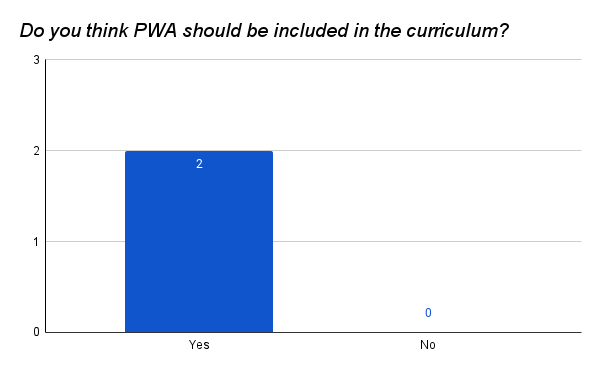
\includegraphics[width=10cm]{img/Results/esq16.png}
    \caption{Answers for ESQ 16}
    \label{fig:res_eduq16}
\end{figure}

ESQ 16 asked respondents whether or not they believe PWA should be included in the curriculum for their courses, results seen in Figure \ref{fig:res_eduq16}. Both respondents answered "Yes" to the question.

% Reset table styling
\setlength{\arrayrulewidth}{0.5mm}
\setlength{\tabcolsep}{8pt}
\renewcommand{\arraystretch}{1.5}
\newpage

\section{Analysis}
This chapter includes analysis of the collected data.

\subsection{Literature Study}
This section analyses the results of the literature study performed at the start of the research project





\subsection{Developer Survey}
This section contains the analysis of the results gathered from the survey given to application developers. The survey was answered by 16 respondents, which was deemed an acceptable amount for drawing generalized conclusions.

\subsubsection{Part 1 - Personal Details}
The first part of the survey consisted of questions DSQ 1 - DSQ 3.



\subsubsection{Part 2 - Experience}
The second part of the survey consisted of questions DSQ 4 - DSQ 7.




\subsubsection{Part 3 - PWA}
The third part of the survey consisted of questions DSQ 8 - DSQ 16.

\subsubsection{Part 4 - Your Company \& Clients}
The fourth part of the survey consisted of questions DSQ 17 - DSQ 19.

\subsubsection{Part 5 - Mobile Applications}
The fifth and final part of the survey consisted of one multi-part question, DSQ 20.





\subsection{Education Survey}
This section contains the analysis of the results gathered from the survey given to lecturers in higher education.

\subsubsection{Part 1 - Personal Details}

\subsubsection{Part 2 - Mobile Applications}

\subsubsection{Part 3 - PWA}


\newpage

\section{Discussion}
Here you discuss your findings and if your problem has been answered. Think of the project as a feedback loop. You define a problem, find a method of approaching it, conduct the study or experiment, and gather data. The data is then used to answer your problem, thus creating the loop. \\

You shall also discuss how your findings relate to what others have done in the field of study. Are your results similar to the findings in the related work you described in the Chapter 3? What is the impact of limitations? How generalizable are the findings? \\

This chapter is typically written in the present tense, while the previous chapters typically are written in past tense.

\newpage

\section{Conclusions}
In this chapter you end your report with a conclusion of your findings.  \\

\noindent What are the results of your thesis project? Try to relate the results to the questions and problem. Did you bridge the knowledge gap? \\

\noindent Are your results relevant for science, industry or society as discussed in you motivation in the Introduction Chapter? How general are your results (i.e. can they be applied to other areas/problems as well)? Also, take a critical stance and question if anything in your project could have been done differently to possibly get better results. \\

\subsection{Future Work}
\noindent You cannot do everything within the limited scope of a degree project. Here you discuss what you would do if you had continued working on your project. Are there any open questions that you discovered during the project work that you didn’t have time to investigate? Are there findings from the evaluation/validation that trigger further investigations?


%------------------------------------------------------------------------
%	References. IEEE style is used.
%------------------------------------------------------------------------
\newpage
\hypersetup{urlcolor=black}
%\bibliographystyle{IEEEtran}
%\bibliography{referenser.bib}
\printbibliography[heading=bibintoc]

\newpage
%------------------------------------------------------------------------
%	Appendix
%------------------------------------------------------------------------
\pagenumbering{Alph}
\setcounter{page}{1} % Reset page numbering for Appendix
\appendix

% Additional appendix styling
\setlength{\parindent}{0pt}
\setlength{\arrayrulewidth}{0.3mm}
\setlength{\tabcolsep}{4pt}
\renewcommand{\arraystretch}{1.5}

\section{Appendix A - Developer Survey}
\textbf{\textit{Part 1 - Personal Details}}

\textbf{In which country do you work?} *

\quad

\textbf{Company name}

\quad

\textbf{Your age} *

\quad

\quad

\textbf{\textit{Part 2 - Experience}}

\textbf{How many years have you worked as a developer?} \textit{single-choice} *
\begin{itemize}
    \item Less than 5 years
    \item 5 - 9 years
    \item 10 - 14 years
    \item More than 15 years
\end{itemize}

\textbf{Pick one; what Best describes your current profession?} \textit{single-choice} *
\begin{itemize}
    \item iOS developer
    \item Android developer
    \item Web developer
    \item Cross-platform developer
\end{itemize}

\textbf{What type of applications have you previously developed or worked on?}
\begin{itemize}
    \item Native iOS
    \item Native Android
    \item Cross-platform / hybrid app
    \item PWA
    \item Regular web app
\end{itemize}

\textbf{Have you ever worked with any of the following cross-platform frameworks?}
\begin{itemize}
    \item React Native
    \item Flutter
    \item PhoneGap / Cordova
    \item Xamarin
    \item Ionic
    \item Other:
\end{itemize}
\quad

\textbf{\textit{Part 3 - PWA}}

\textbf{How good is your knowledge of PWAs?}  \textit{single-choice} *

\begin{tabular}{ccccc}
    None & & & & Very good \\
    \hline
    \multicolumn{1}{|c|}{1} & \multicolumn{1}{c|}{2} & \multicolumn{1}{c|}{3} & \multicolumn{1}{c|}{4} & \multicolumn{1}{c|}{5} \\
     \hline
\end{tabular}

\quad

\quad

\textbf{Would you consider developing a PWA in the future?} \textit{single-choice} *
\begin{itemize}
    \item Yes
    \item No
    \item Other:
\end{itemize}

\textbf{Is there anything that makes you prefer other cross-platform solutions over PWA?}

\quad

\textbf{Is there anything that makes you prefer developing natively over PWA?}

\quad

\textbf{Have you ever encountered any of the following problems with PWAs?}
\begin{itemize}
    \item Not all hardware features were accessible, such as Bluetooth or NFC
    \item Not all software features were accessible, such as contacts or SMS
    \item Battery consumption was higher
    \item Poor support for legacy devices and browsers
    \item Poor support on iOS devices
    \item Not distributable on mobile app stores
    \item Other:
\end{itemize}

\textbf{When was the last time you encountered any of the problems above?} \textit{single-choice}
\begin{itemize}
    \item 2016
    \item 2017
    \item 2018
    \item 2019
    \item 2020
    \item 2021
\end{itemize}

\textbf{What is your opinion on PWA as a development technique today?} *

\textit{For example: "It is a somewhat decent cross-platform solution, but until it has proper iOS support I will not consider it".}

\quad

\textbf{How much do you agree with this statement: "PWA is the future of mobile app development"} \textit{single-choice}  *

\begin{tabular}{ccccc}
    Strongly disagree & & & & Strongly agree \\
    \hline
    \multicolumn{1}{|c|}{1} & \multicolumn{1}{c|}{2} & \multicolumn{1}{c|}{3} & \multicolumn{1}{c|}{4} & \multicolumn{1}{c|}{5} \\
     \hline
\end{tabular}

\quad

\quad

\textbf{If you disagree, how do you think PWAs need to change before the statement becomes true?}

\quad

\quad

\textbf{\textit{Part 4 - Your Company \& Clients}}

\textbf{Has a client ever asked for a PWA?} \textit{single-choice} *
\begin{itemize}
    \item Yes
    \item No
    \item I do not know
\end{itemize}

\textbf{Have you ever proposed PWA as a solution to a client?} *
\begin{itemize}
    \item Yes
    \item No
\end{itemize}

\textbf{What type of apps does your company offer?} *
\begin{itemize}
    \item Native apps
    \item Hybrid apps
    \item Cross-platform apps
    \item PWAs
    \item Web apps
    \item Other:
\end{itemize}
\quad

\textbf{\textit{Part 5 - Mobile Applications}}

\textbf{Please rank the importance of the following features and qualities of mobile apps}
\begin{tabular}{|p{3cm}|p{1.7cm}|p{1.7cm}|p{1.6cm}|p{1.7cm}|p{1.6cm}|p{1.4cm}|}
  \hline
     & Not at all important  & Slightly important  &  Important & Fairly important  & Very important  & No opinion \\
  \hline
  Available on app stores   &   &   &   &   &   &  \\
  \hline
  Installable (app store or web download)   &   &   &   &   &   & \\
  \hline
   Push notifications  &   &   &   &   &   & \\
  \hline
   Background sync   &   &   &   &   &   & \\
  \hline
   High performance  &   &   &   &   &   & \\
  \hline
   Low battery usage  &   &   &   &   &   & \\
  \hline
   Usable while offline &   &   &   &   &   & \\
  \hline
   Cross-platform  &   &   &   &   &   & \\
  \hline
   Discoverable from web-search  &   &   &   &   &   & \\
  \hline
\end{tabular}

\quad

\textbf{\textit{Final thoughts}}

\textbf{If you have any feedback about the survey or just want to add some final thoughts, please do so here}

\newpage
\section{Appendix B - Education Survey}
\textbf{\textit{Part 1 - Personal Details}}

\textbf{In which country do you work?} *

\quad

\textbf{Where do you work?}

\textit{The name of you university, polytechnic, college, etc.}

\quad

\textbf{What is your age?}  \textit{single-choice} *
\begin{itemize}
    \item 20 - 29
    \item 30 - 39
    \item 40 - 49
    \item 50 - 59
    \item 60 or above
\end{itemize}


\textbf{In which of the following subjects do you teach?} *
\begin{itemize}
    \item Web development
    \item Web design
    \item Mobile app development
    \item Mobile app design
    \item Other:
\end{itemize}

\textbf{How long have you been teaching in these subjects?} \textit{single-choice} *
\begin{itemize}
    \item Less than 5 years
    \item 5 - 9 years
    \item More than 10 years
\end{itemize}

\quad

\quad

\textbf{\textit{Part 2 - Mobile Applications}}

\textbf{What type of applications do your courses cover?}
\begin{itemize}
    \item Native iOS
    \item Native Android
    \item Web
    \item Cross-platform / hybrid
    \item Other:
\end{itemize}

\textbf{If your courses do not cover cross-platform apps, do you think it should be covered in the future?}
\begin{itemize}
    \item Yes
    \item No
    \item No opinion
\end{itemize}

\textbf{If your courses do cover cross-platform apps, does it cover any of the following frameworks?}
\begin{itemize}
    \item Xamarin
    \item React Native
    \item Flutter
    \item PhoneGap / Cordova
    \item Ionic
    \item Other:
\end{itemize}

\textbf{Please rank the importance of the following features and qualities of mobile apps}

\begin{tabular}{|p{3cm}|p{1.7cm}|p{1.7cm}|p{1.6cm}|p{1.7cm}|p{1.6cm}|p{1.4cm}|}
  \hline
     & Not at all important  & Slightly important  &  Important & Fairly important  & Very important  & No opinion \\
  \hline
  Available on app stores   &   &   &   &   &   &  \\
  \hline
  Installable (app store or web download)   &   &   &   &   &   & \\
  \hline
   Push notifications  &   &   &   &   &   & \\
  \hline
   Background sync   &   &   &   &   &   & \\
  \hline
   High performance  &   &   &   &   &   & \\
  \hline
   Low battery usage  &   &   &   &   &   & \\
  \hline
   Usable while offline &   &   &   &   &   & \\
  \hline
   Cross-platform  &   &   &   &   &   & \\
  \hline
   Discoverable from web-search  &   &   &   &   &   & \\
  \hline
\end{tabular}

\quad

\quad

\textbf{\textit{Part 3 - PWA}}

\textbf{How good is your knowledge of PWAs?}  \textit{single-choice} *

\begin{tabular}{ccccc}
    None & & & & Very good \\
    \hline
    \multicolumn{1}{|c|}{1} & \multicolumn{1}{c|}{2} & \multicolumn{1}{c|}{3} & \multicolumn{1}{c|}{4} & \multicolumn{1}{c|}{5} \\
     \hline
\end{tabular}

\quad

\quad

\textbf{Is PWA mentioned in the required literature in any of your courses?} \textit{single-choice} *
\begin{itemize}
    \item Yes
    \item No
    \item I do not know
\end{itemize}

\textbf{Is PWA part of the curriculum in any of your courses?} \textit{single-choice} *
\begin{itemize}
    \item Yes
    \item No
\end{itemize}

\textbf{If not, please give a short explanation}

\textit{For example: "The course does not cover cross-platform development, only native Android"}

\quad

\textbf{Has it ever been requested that PWA be included in the curriculum?} \textit{single-choice} *
\begin{itemize}
    \item Yes
    \item No
\end{itemize}

\textbf{If yes, from whom?}

\textit{For example: "A student expressed interest in learning more about it after they learned that 'Twitter Lite' is a PWA".}

\quad

\textbf{Do you think PWA should be included in the curriculum?}
\begin{itemize}
    \item Yes
    \item No
    \item No opinion
\end{itemize}

\quad

\quad

\textbf{\textit{Final thoughts}}

\textbf{If you have any feedback about the survey or just want to add some final thoughts, please do so here}

\newpage
\section{Appendix C - DSQ 20 Diagrams}

\begin{figure}[ht!]
    \centering
    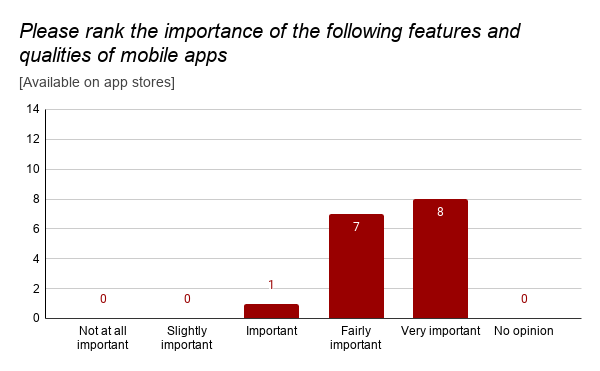
\includegraphics[width=10cm]{img/Results/dsq20_1.png}
    \caption{Answers for DSQ 20, part 1}
    \label{fig:res_devq20_1}
\end{figure}

\begin{figure}[ht!]
    \centering
    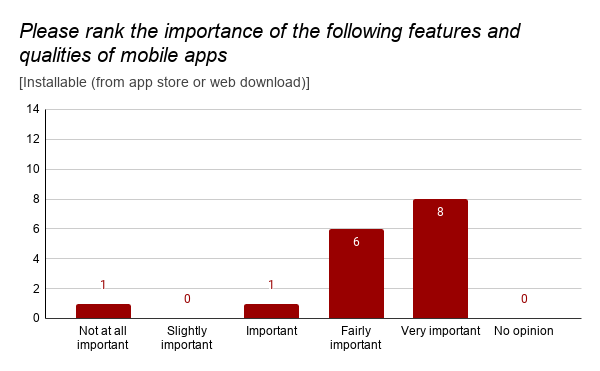
\includegraphics[width=10cm]{img/Results/dsq20_2.png}
    \caption{Answers for DSQ 20, part 2}
    \label{fig:res_devq20_2}
\end{figure}

\begin{figure}[ht!]
    \centering
    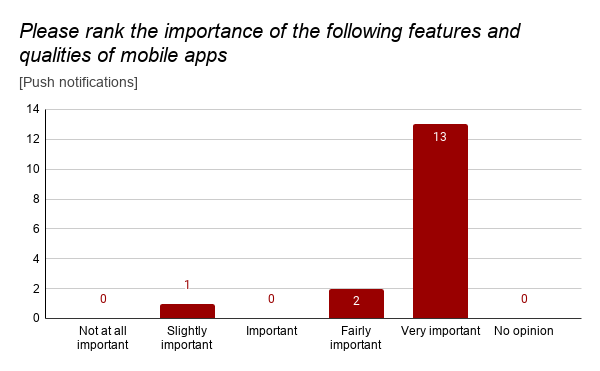
\includegraphics[width=10cm]{img/Results/dsq20_3.png}
    \caption{Answers for DSQ 20, part 3}
    \label{fig:res_devq20_3}
\end{figure}
\newpage

\begin{figure}[ht!]
    \centering
    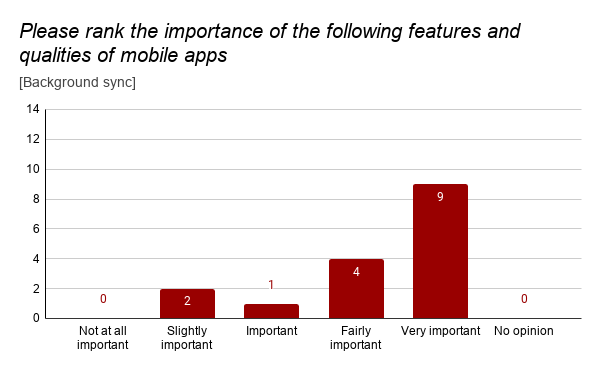
\includegraphics[width=10cm]{img/Results/dsq20_4.png}
    \caption{Answers for DSQ 20, part 4}
    \label{fig:res_devq20_4}
\end{figure}

\begin{figure}[ht!]
    \centering
    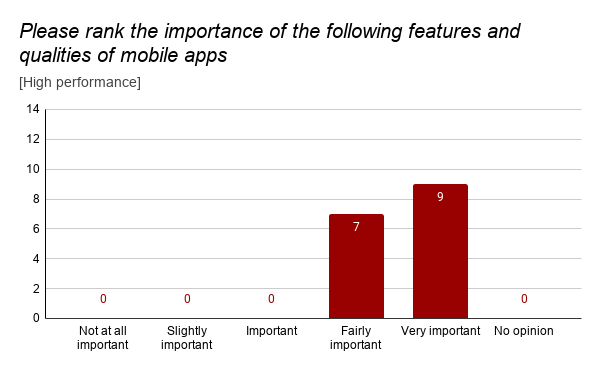
\includegraphics[width=10cm]{img/Results/dsq20_5.png}
    \caption{Answers for DSQ 20, part 5}
    \label{fig:res_devq20_5}
\end{figure}

\begin{figure}[ht!]
    \centering
    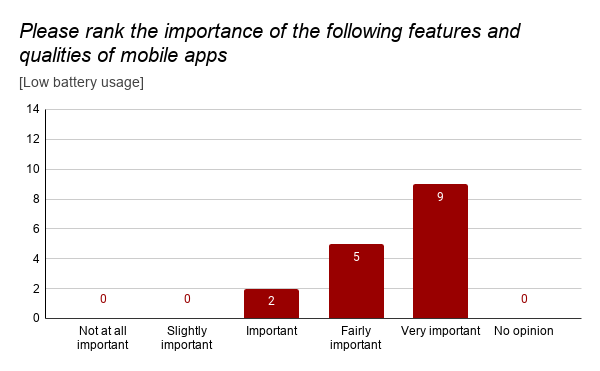
\includegraphics[width=10cm]{img/Results/dsq20_6.png}
    \caption{Answers for DSQ 20, part 6}
    \label{fig:res_devq20_6}
\end{figure}
\newpage

\begin{figure}[ht!]
    \centering
    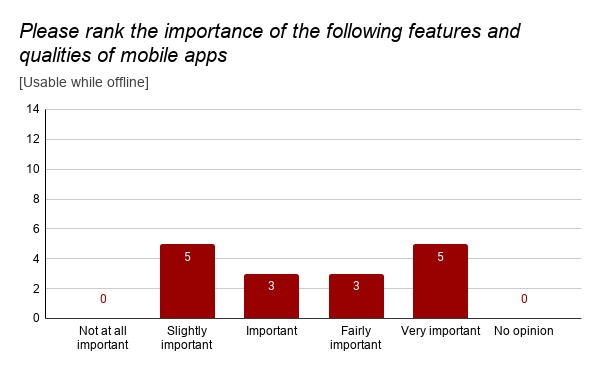
\includegraphics[width=10cm]{img/Results/dsq20_7.png}
    \caption{Answers for DSQ 20, part 7}
    \label{fig:res_devq20_7}
\end{figure}

\begin{figure}[ht!]
    \centering
    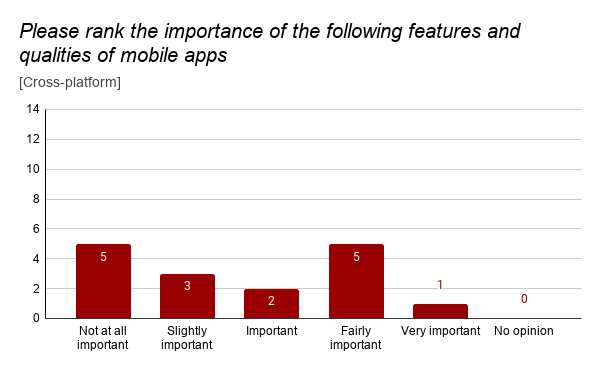
\includegraphics[width=10cm]{img/Results/dsq20_8.png}
    \caption{Answers for DSQ 20, part 8}
    \label{fig:res_devq20_8}
\end{figure}

\begin{figure}[ht!]
    \centering
    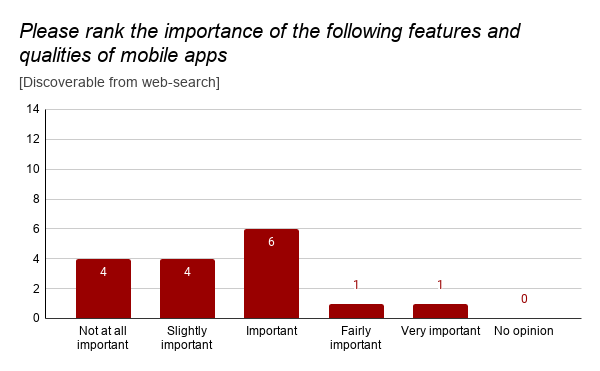
\includegraphics[width=10cm]{img/Results/dsq20_9.png}
    \caption{Answers for DSQ 20, part 9}
    \label{fig:res_devq20_9}
\end{figure}

\newpage

\section{Appendix D - ESQ 9 Diagrams}
\begin{figure}[ht!]
    \centering
    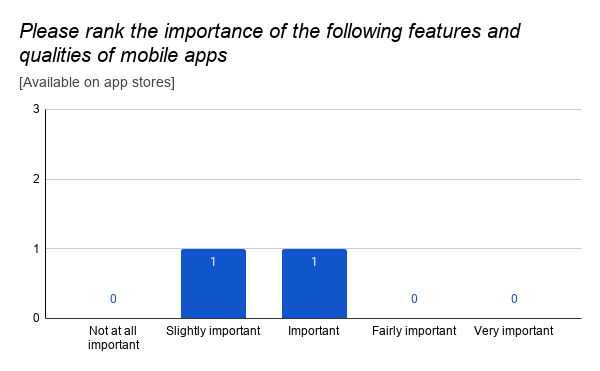
\includegraphics[width=10cm]{img/Results/esq9_1.png}
    \caption{Answers for ESQ 9, part 1}
    \label{fig:res_eduq9_1}
\end{figure}

\begin{figure}[ht!]
    \centering
    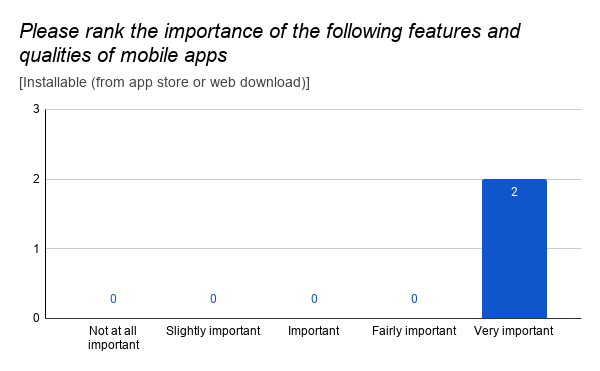
\includegraphics[width=10cm]{img/Results/esq9_2.png}
    \caption{Answers for ESQ 9, part 2}
    \label{fig:res_eduq9_2}
\end{figure}

\begin{figure}[ht!]
    \centering
    \includegraphics[width=10cm]{img/Results/esq9_3.png}
    \caption{Answers for ESQ 9, part 3}
    \label{fig:res_eduq9_3}
\end{figure}

\begin{figure}[ht!]
    \centering
    \includegraphics[width=10cm]{img/Results/esq9_4.png}
    \caption{Answers for ESQ 9, part 4}
    \label{fig:res_eduq9_4}
\end{figure}

\begin{figure}[ht!]
    \centering
    \includegraphics[width=10cm]{img/Results/esq9_5.png}
    \caption{Answers for ESQ 9, part 5}
    \label{fig:res_eduq9_5}
\end{figure}

\begin{figure}[ht!]
    \centering
    \includegraphics[width=10cm]{img/Results/esq9_6.png}
    \caption{Answers for ESQ 9, part 6}
    \label{fig:res_eduq9_6}
\end{figure}

\begin{figure}[ht!]
    \centering
    \includegraphics[width=10cm]{img/Results/esq9_7.png}
    \caption{Answers for ESQ 9, part 7}
    \label{fig:res_eduq9_7}
\end{figure}

\begin{figure}[ht!]
    \centering
    \includegraphics[width=10cm]{img/Results/esq9_8.png}
    \caption{Answers for ESQ 9, part 8}
    \label{fig:res_eduq9_8}
\end{figure}

\begin{figure}[ht!]
    \centering
    \includegraphics[width=10cm]{img/Results/esq9_9.png}
    \caption{Answers for ESQ 9, part 9}
    \label{fig:res_eduq9_9}
\end{figure}
\end{document}
